% !TeX program = xelatex
% !TeX encoding = UTF-8
\documentclass{MathorCupmodeling}
\usepackage{mwe,color,float}
\usepackage[linesnumbered,ruled]{algorithm2e}
\usepackage{setspace}
\usepackage{pdfpages}
\usepackage{graphicx}
\extrafloats{100}
\bianhao{MCB2301959}
\tihao{A}
\timu{\textbf{基于卷积神经网络CNN图像特征提取的SVM坑洼道路检测与识别}}
\keyword{计算机视觉;卷积神经网络;支持向量机;特征提取;模型融合;可视化多维评估}
\begin{document}
	\begin{abstract}
		坑洼道路的高效检测可有效地推进无人驾驶、地质勘探、航天科学等领域的研究与应用。由于道路图像的环境背景复杂及多变性,传统算法难以提取有效特征,效果较差。因此,本文旨在建立基于卷积神经网络图像特征提取的 SVM 模型,对坑洼道路进行检测与识别。
		
		{\heiti 针对问题一},需要提取给定图像的特征,建立一个用于识别其为正常或是坑洼道路的识别率高、速度快、分类准确的模型。首先,对图像文件\textbf{预处理},包括\textbf{人为再分类},对标记错误的进行\textbf{修正},或\textbf{剔除异常图像};再将两类图像置于各子文件中。其次,从\textbf{机理层面}对正常与坑洼道路进行比较分析,包括\textbf{原图、热力图、RGB与灰度直方图的对比、边缘与轮廓检测、阈值分割},从而有效地提取出\textbf{图像特征}。之后,利用\textbf{opencv-python}读取图像,并加入\textbf{try-except异常处理}语块,\textbf{防止破损文件污染模型};此外,计算出正常与坑洼道路的个数比值为$\boldsymbol{6.32}$,即\textbf{数据集类别不平衡},因此采用\textbf{基于抽样的方法平衡化};之后,以$\boldsymbol{8:2}$的比例划分数据集为\textbf{训练集与测试集};考虑到现有的图像未能较全面地展现特征,因此\textbf{对训练集采用高斯、双边滤波,旋转处理进行图像增强}。随后,建立支持向量机、卷积神经网络的单一模型,但由于\textbf{CNN中softmax函数的局限性},因而,\textbf{利用卷积神经网络对图像信息的特征进行提取},依据上述分析,设定其输入层、卷积层、激活层、池化层、全连接层参数,具体见\textcolor{blue}{\cref{fig:CNN模型架构}};在此基础上,建立\textbf{支持向量机分类模型},对道路类别进行分类。

		{\heiti 针对问题二},需要对问题一的模型进行训练,并进行多维度的评估分析,保证模型的准确性、快速性及普适性。因此,对问题一所建立的模型进行训练与测试,并从\textbf{模型耗时、准确率、分类报告、五折交叉验证,混淆矩阵、ROC/AUC曲线}进行多维度评价。模型\textbf{准确率在$\boldsymbol{95\,\%}$的置信水平下达到$\boldsymbol{\left(90\pm 8\right)\,\%}$};其\textbf{精确率、召回率、F1分数值在各维度下均于$\boldsymbol{88\,\%}$及以上};\textbf{ROC/AUC曲线靠近图的左上角,曲线下面积达到$\boldsymbol{0.90}$},具体见\textcolor{blue}{\cref{fig:CNN-SVM分类报告图}}\textasciitilde\textcolor{blue}{\cref{fig:CNN-SVM精确率召回率曲线}}。此外,还将其与单一模型进行多维度对比,\textbf{准确率最高可提升$\boldsymbol{3\,\%}$},模型提升效果良好,结果具体见\textcolor{blue}{\cref{tab:模型效果对比}}。

		{\heiti 针对问题三},需要利用上述已建立的模型,对未知数据集图像进行分类,并保存结果。经过读取模型、读取数据、数据集预处理、预测得出模型\textbf{在4942张图像中,识别出坑洼道路为3765张,识别为正常道路为1177张}。
		
		{\heiti 最后},本文对所建立的模型的优缺点进行了中肯的评价、提出了模型的改进措施以及对模型进行了一定推广。
	\end{abstract}

	\pagestyle{empty}
	\tableofcontents
	\newpage
	\pagestyle{fancy}

	\setcounter{page}{1}
	\section{问题的提出}
	\subsection{问题背景}
	坑洼道路的检测与识别工作是推动自动无人驾驶、地质勘探、航天科学及自然灾害等领域研究和应用的不可或缺的计算机视觉任务。然而传统的分类算法往往因坑洼图像的复杂及多变性,不能取得较好的效果。近年来,深度学习邻域技术的发展为坑洼道路的检测、为当前存在的亟待解决的问题提供了新的思想。

	在实际工程应用中,非结构化的坑洼道路检测将遇到复杂多样的环境,例如,道路周围环境存在差异、光照条件变化等,这无疑增加了基于视觉检测道路的难度\textcolor{blue}{\cite{曹江华}}。道路坑洼的检测是实现智能车辆导航的基础,只有快速准确地检测出道路的可行驶区域才能够真正实现自动驾驶。

	深度学习拥有很强的特征提取与表示能力,可从图像中提取重要特征。于坑洼道路检测和识别而言,其可识别坑洼的轮廓、纹理、形态等特征,并将上述特征转换为更易分类的表现形式。在深度学习的基础上,迁移学习、知识蒸馏等技术可进一步提升分类性能以更加准确对新出现的道路图像自动识别。
	\subsection{问题要求}
	\begin{itemize}
		\item {\heiti 初赛:}
		\begin{itemize}
			\item \textbf{问题一:}基于图像文件,提取图像特征,以“正常”和“坑洼”为特征建立一个识别率高、速度快且分类准确的模型。
			\item \textbf{问题二:}对问题一中所建立的模型进行训练,并对其进行多维度的评估分析。
			\item \textbf{问题三:}利用训练模型识别测试集中的坑洼图像,并展分析结果的合理性。
		\end{itemize}
		\item {\heiti 复赛:}
		\begin{itemize}
			\item \textbf{问题一}:建立可以更精准地识别坑洼边缘的模型,以满足道路避障、道路修复等工作的需求。
			\item \textbf{问题二}:依据识别的坑洼边缘,对其面积进行估算,计算各坑洼占其图像面积的百分比。
		\end{itemize}
	\end{itemize}
	\section{问题的分析}
	\subsection{问题的整体分析}
	该题是一个基于计算机视觉的坑洼道路的图像数据分析、预测类问题。

	\textbf{从分析目的看},本题需要分析道路图像并提取其特征,并建立一个识别率高、速度快、分类准确的模型,用以准确判断道路是正常或是坑洼。因此本题需要完成以下两方面任务:{\heiti 其一},分析、研究不同道路图像的特征并归类总结,为后续模型的建立提供支撑。{\heiti 其二},根据上述分析,建立合适的模型,通过对道路图像特征识别,判断道路是否正常。确保模型的准确性、快速性及普适性。

	\textbf{从图像数据特征看},本题的道路图像具有数量多,环境等情况复杂,以及坑洼形态多样等特征,极大地增加的模型学习的难度。因此优先考虑深度学习的方法,利用其强大的特征提取与表示能力,对道路图像进行特征提取,再建立合适的模型进行分类预测。

	\textbf{从模型的选择看},本题图像数量多,特征复杂,且需要对道路图像做出准确分类。同时结合图像数据特征的分析,我们考虑结合图像增强技术建立深度学习的特征提取与分类的机器学习模型。

	\textbf{从编程软件的选择看},本题为图像大数据分析类,需要对大量的图片数据进行分析,并依据设问建立合适的模型,对正常及坑洼道路的图像进行分类预测,因此我们选择使用Python Jupyter对问题进行求解,其交互式的编程范式及轻量化,方便且高效。

	\subsection{各问题逐一分析}
	\begin{itemize}
		\item \textbf{问题一}:其核心目的在于{\heiti 结合给定的图像数据集,对其进行特征的提取,从而建立一个用于识别其为正常道路或是坑洼道路的模型}。此外,该模型需要具有{\heiti 识别率高、速度快、分类准确}的特点。首先,需要对图像文件进行预处理,包括人为再分类、文件夹分类,对标记错误的图像进行修正,并剔除异常的图像。之后从机理层面对正常与坑洼道路进行比较分析,包括原图、热力图、RGB直方图、灰度直方图对比、边缘及轮廓检测、以及阈值分割,从而有效地提取出图像特征。随后,对图像数据进行预处理,将划分标记好的文件读入内存中,分析各类占比,对数据集进行平衡化,在此基础上划分数据集为训练集及测试集,考虑到图像文件并未能很好地全面展现特征,因此考虑对训练集数据进行增强,增加模型的学习样本。完成上述步骤后,即开始建立模型。我们从三方面考虑,其一,利用主成分分析法对数据进行降维,再建立支持向量机模型,同时加入网格调优。其二,建立卷积神经网络深度学习模型,设定其输入层、卷积层、激活层、池化层、全连接层参数。其三,考虑到单一模型存在一定局限性,因此建立基于卷积神经网络图像特征提取的SVM模型,利用CNN网络对图像数据进行特征提取,再利用支持向量机对其进行分类。
		\item \textbf{问题二}:其核心目的在于{\heiti 对问题一的模型进行训练,并对其进行多维度的评估分析,以保证模型的准确性、快速性及普适性}。因此,我们首先对问题一中所建立的前两个模型进行学习,并对其进行评估分析,主要从分类报告分析。之后将已训练好的CNN模型用于图像特征的提取,在此基础上再训练SVM模型,优化参数,并对其进行评估分析。本文用于评估模型效果的主要方法有:时间、准确率、损失值、分类报告、混淆矩阵、ROC/AUC曲线、精确率与召回率曲线、交叉验证。最后,对模型进行整体评价,选择出最优模型。
		\item \textbf{问题三}:其核心目的在于{\heiti 利用上述已建立的模型,对未知数据集图像进行分类,并保存结果}。因此,我们需要读取问题一、二中所建立及训练好的模型,对未知数据集进行预测,注意分类标识的顶柜,同时也需注意避免文件名与被预测值错位,并将其文件名与对应的类别保存好。
	\end{itemize}
	\subsection{本文思路}
	为了便于理清思路,绘制出本文解决问题的流程图,如\textcolor{blue}{\cref{fig:流程图}}所示。
	\begin{figure}[H]
		\centering
		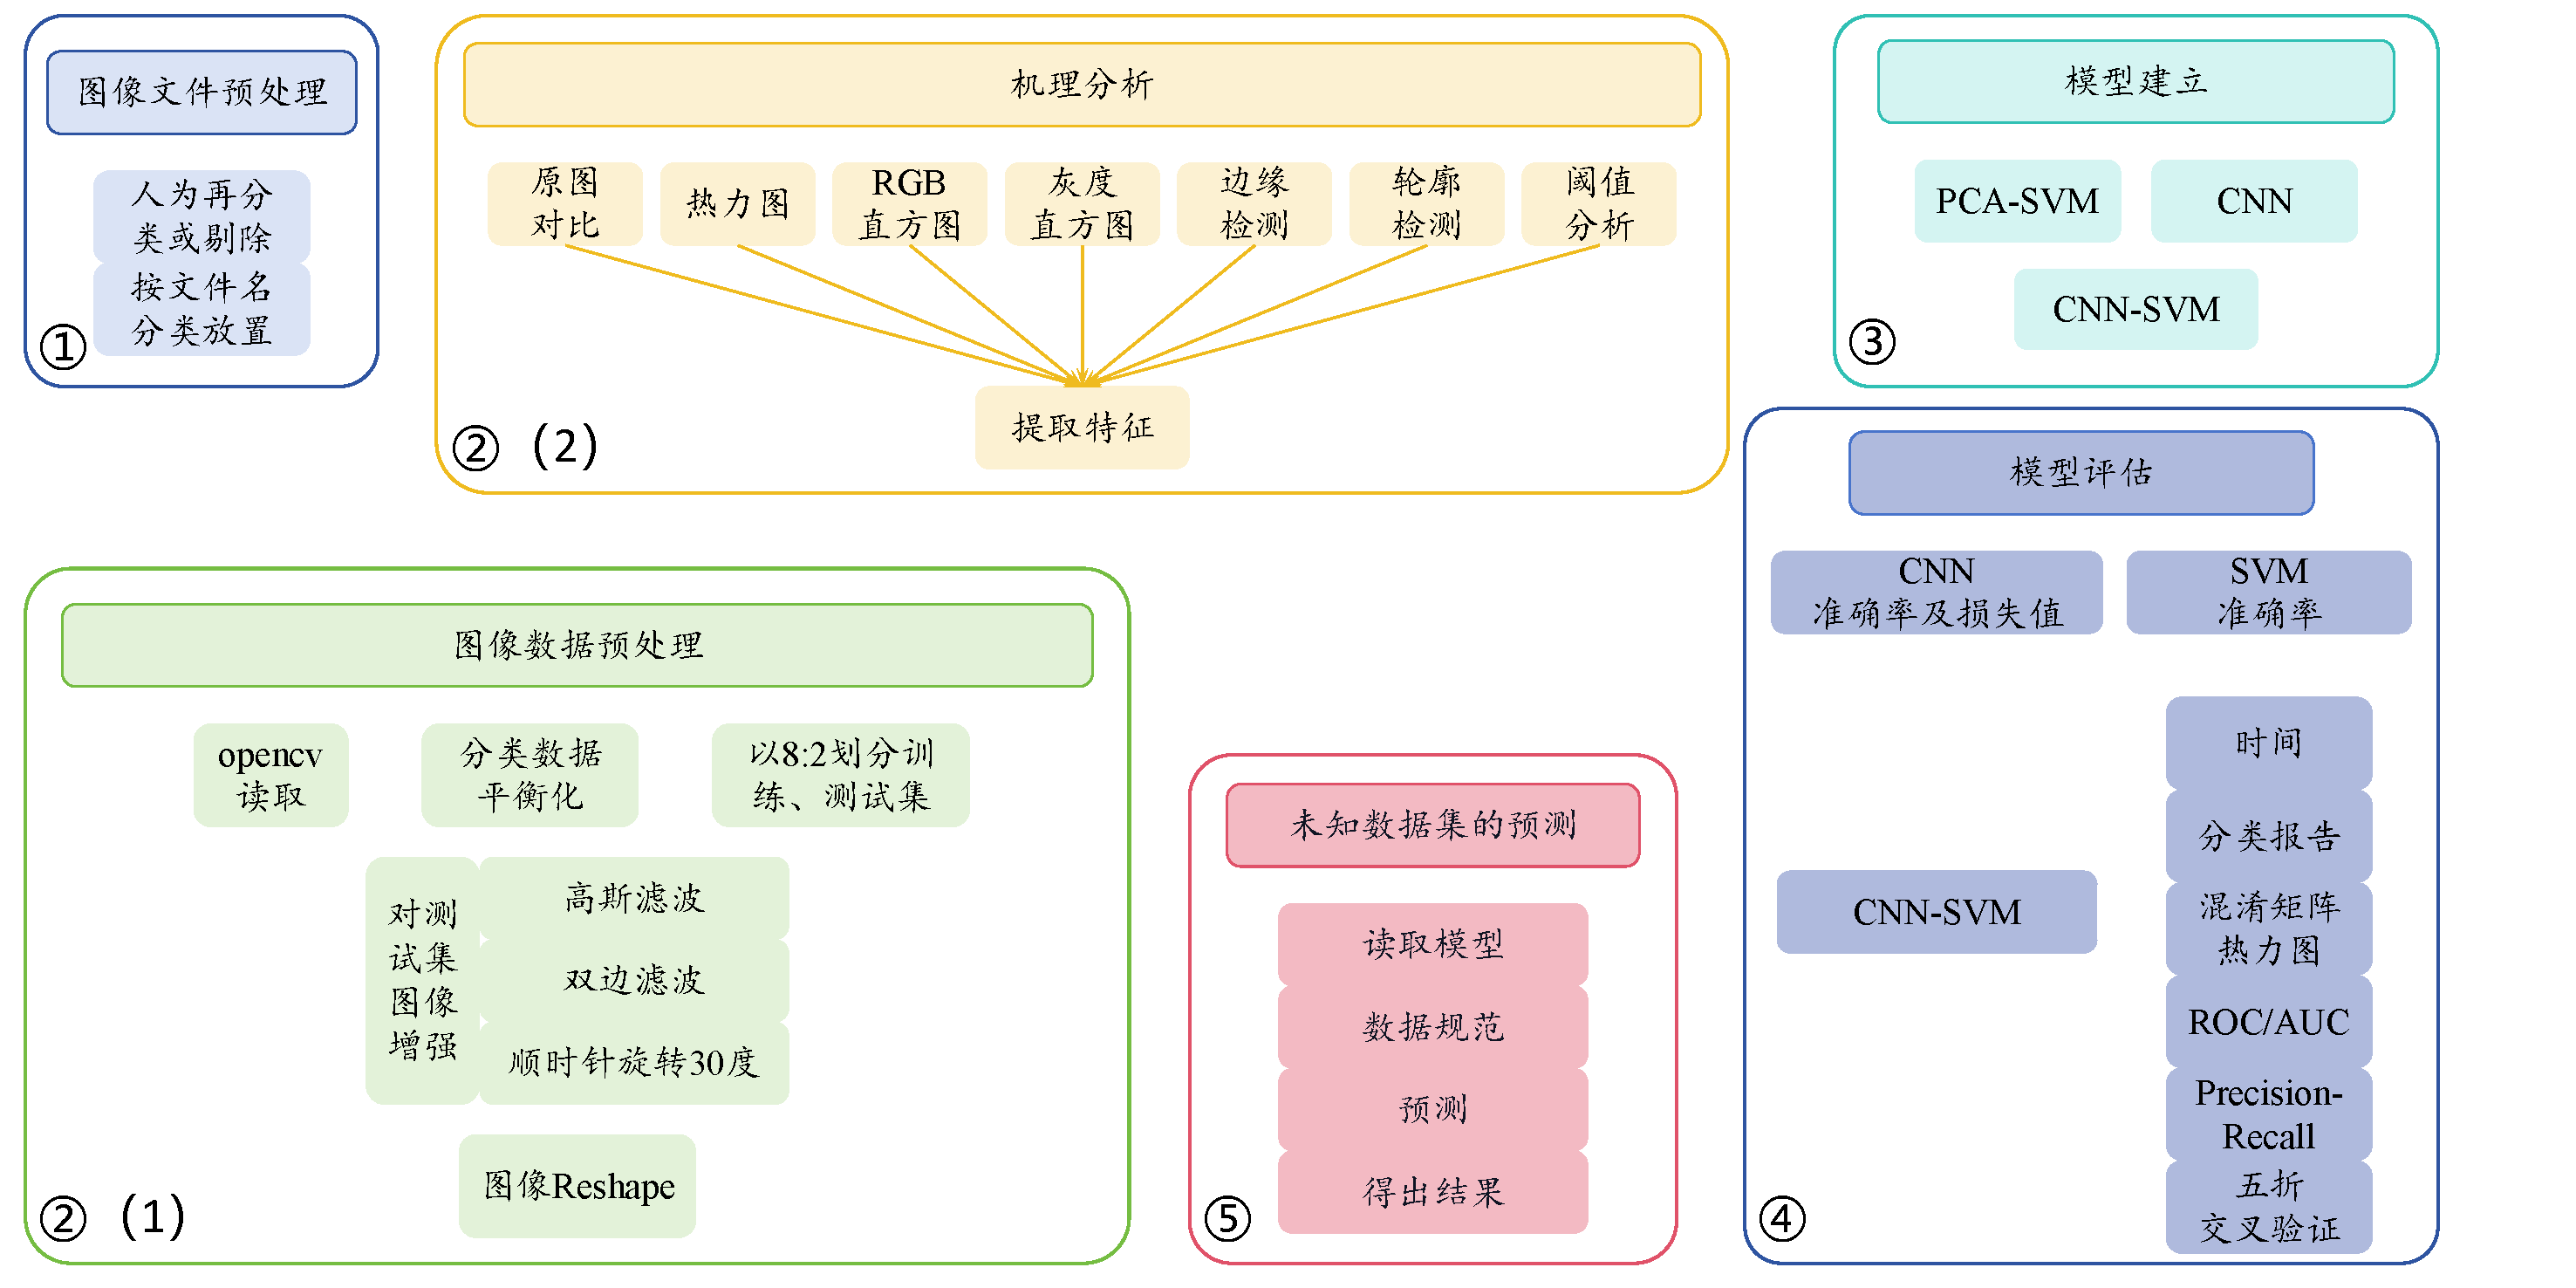
\includegraphics[scale=0.32]{流程图.pdf}
		\caption{流程图}
		\label{fig:流程图}
	\end{figure}
	\section{符号说明}
	\begin{center}
		\scalebox{0.9}{
		\begin{tabularx}{0.7\textwidth}{c@{\hspace{1pc}}|@{\hspace{2pc}}X}
			\Xhline{0.08em}
			\textbf{符号} & \multicolumn{1}{c}{\textbf{符号说明}}\\
			\Xhline{0.05em}
			$X$ & 图像横轴像素点的像素值\\
			$Y$ & 图像纵轴像素点的像素值\\
			$I_f$ & 滤波后的图像像素值\\
			$I$ & 原始图像像素值\\
			$G_s$ & 归一化权重\\
			$\Omega$ & 滤波邻域窗口\\
			$F_s$ & 空间域核函数\\
			$F_f$ & 像素值域核函数\\
			$E\left(x\right)$ & 数据均值\\
			$\lambda_n$ & 协方差矩阵特征值\\
			$\boldsymbol{u}$ & 协方差矩阵特征向量\\
			$C$ & SVM惩罚系数\\
			$S$ & 池化区域面积\\
			$N_{\text{TruePredict}}$ & 预测正确样本数\\
			$N_{\text{Predict}}$ & 预测样本总数\\
			\Xhline{0.08em}
		\end{tabularx}}
	\end{center}

	\textbf{注:}这里并未列出其余变量,这是由于它们在不同小节处有不同的含义,同时该表中也未列出专有定义的变量,这些变量在使用时会在相应位置进行详细说明。
	\section{模型的假设}
	\begin{itemize}
		\item \textbf{假设一}:所给数据集存在因某些原因而标注异常的图像数据的现象;
		\item \textbf{假设二}:所给数据集未能完整地表现出分类的特征。
	\end{itemize}
	\section{模型的建立与求解}
	\subsection{图像文件预处理}\label{图像文件预处理}
	该题附件1为“data.zip”,共包含301张图片,且均为“jpg”格式,且在文件名中进行了标注。其中,文件名中包含“normal”字符的表示正常道路,共266张,包含“potholes”字符的为坑洼道路,共35张。考虑到数据的标注严谨性,我们首先对其进行人为再分类,将标注异常的进行重新标注或剔除。此外,为方便后续模型的分析、建立与求解,我们将“normal”与“potholes”图像文件置于“DATA”文件下的“normal”及“potholes”文件夹中。
	\subsubsection{人为再分类}
	考虑到数据的标注严谨性,我们首先对其进行人为再分类,将标注异常的进行重新标注或剔除。对于所给数据集,我们筛选出了以下几张图片,其标注存在问题,需要进行重新标注或剔除,如\textcolor{blue}{\cref{fig:异常图片}}所示,图中所标注的为该图像的原始文件名。
	\begin{figure}[H]
		\centering
		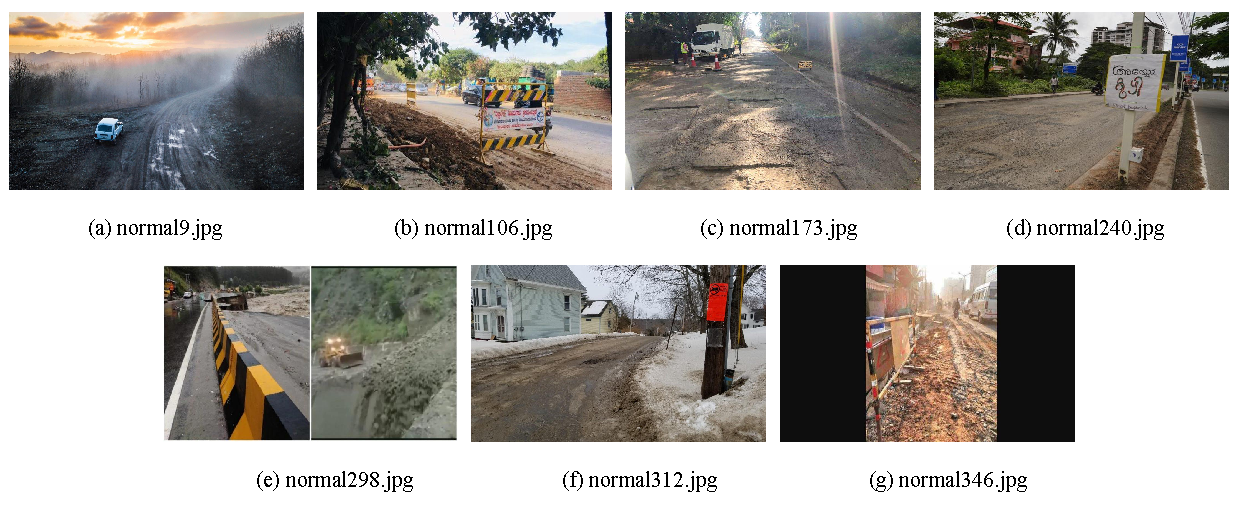
\includegraphics[scale=0.8]{异常图片.pdf}
		\caption{标注异常图片}
		\label{fig:异常图片}
	\end{figure}

	对于上述“(e) normal298.jpg”文件,我们选择剔除,其余划分为“potholes”类。具体处理见\textcolor{blue}{\cref{tab:异常图片处理}}。表中“potholes”代表将该问价视为坑洼道路,而“删除”代表将该文件删除,不参与后续模型的分析、建立、训练等。

\begin{table}[H]
	\centering
	\caption{异常标注图片的处理}
	\scalebox{0.9}{
	  \begin{tabular}{ccc}
	  \toprule
	  \textbf{编号}    & \textbf{原文件名}  & \textbf{处理方式} \\
	  \midrule
	  a     & normal9.jpg & potholes \\
	  b     & normal106.jpg & potholes \\
	  c     & normal173.jpg & potholes \\
	  d     & normal240.jpg & potholes \\
	  e     & normal298.jpg & 删除 \\
	  f     & normal312.jpg & potholes \\
	  g     & normal346.jpg & potholes \\
	  \bottomrule
	  \end{tabular}}
	\label{tab:异常图片处理}
\end{table}
	\subsubsection{文件夹分类}
	为了后续模型的分析、建立与求解,我们将“normal”与“potholes”图像文件置于“DATA”文件下的“normal”及“potholes”文件夹中,作为二分类的数据集。该处理我们使用Python的os及shutil库进行处理,首先指定根目录为“DATA”,再在其下创建“normal”与“potholes”文件夹,之后读取“DATA”文件夹下的所有文件,若文件名中含有“normal”字符,则将其放置于“normal”文件夹中,否则放置于“potholes”文件夹中。具体处理代码见\textbf{附录-C.1,Data Preprocessing [数据预处理]}。
	
	这里,我们可以大致观测数据集图像,如\textcolor{blue}{\cref{fig:图像数据观测}}所示。
	\begin{figure}[H]
		\centering
		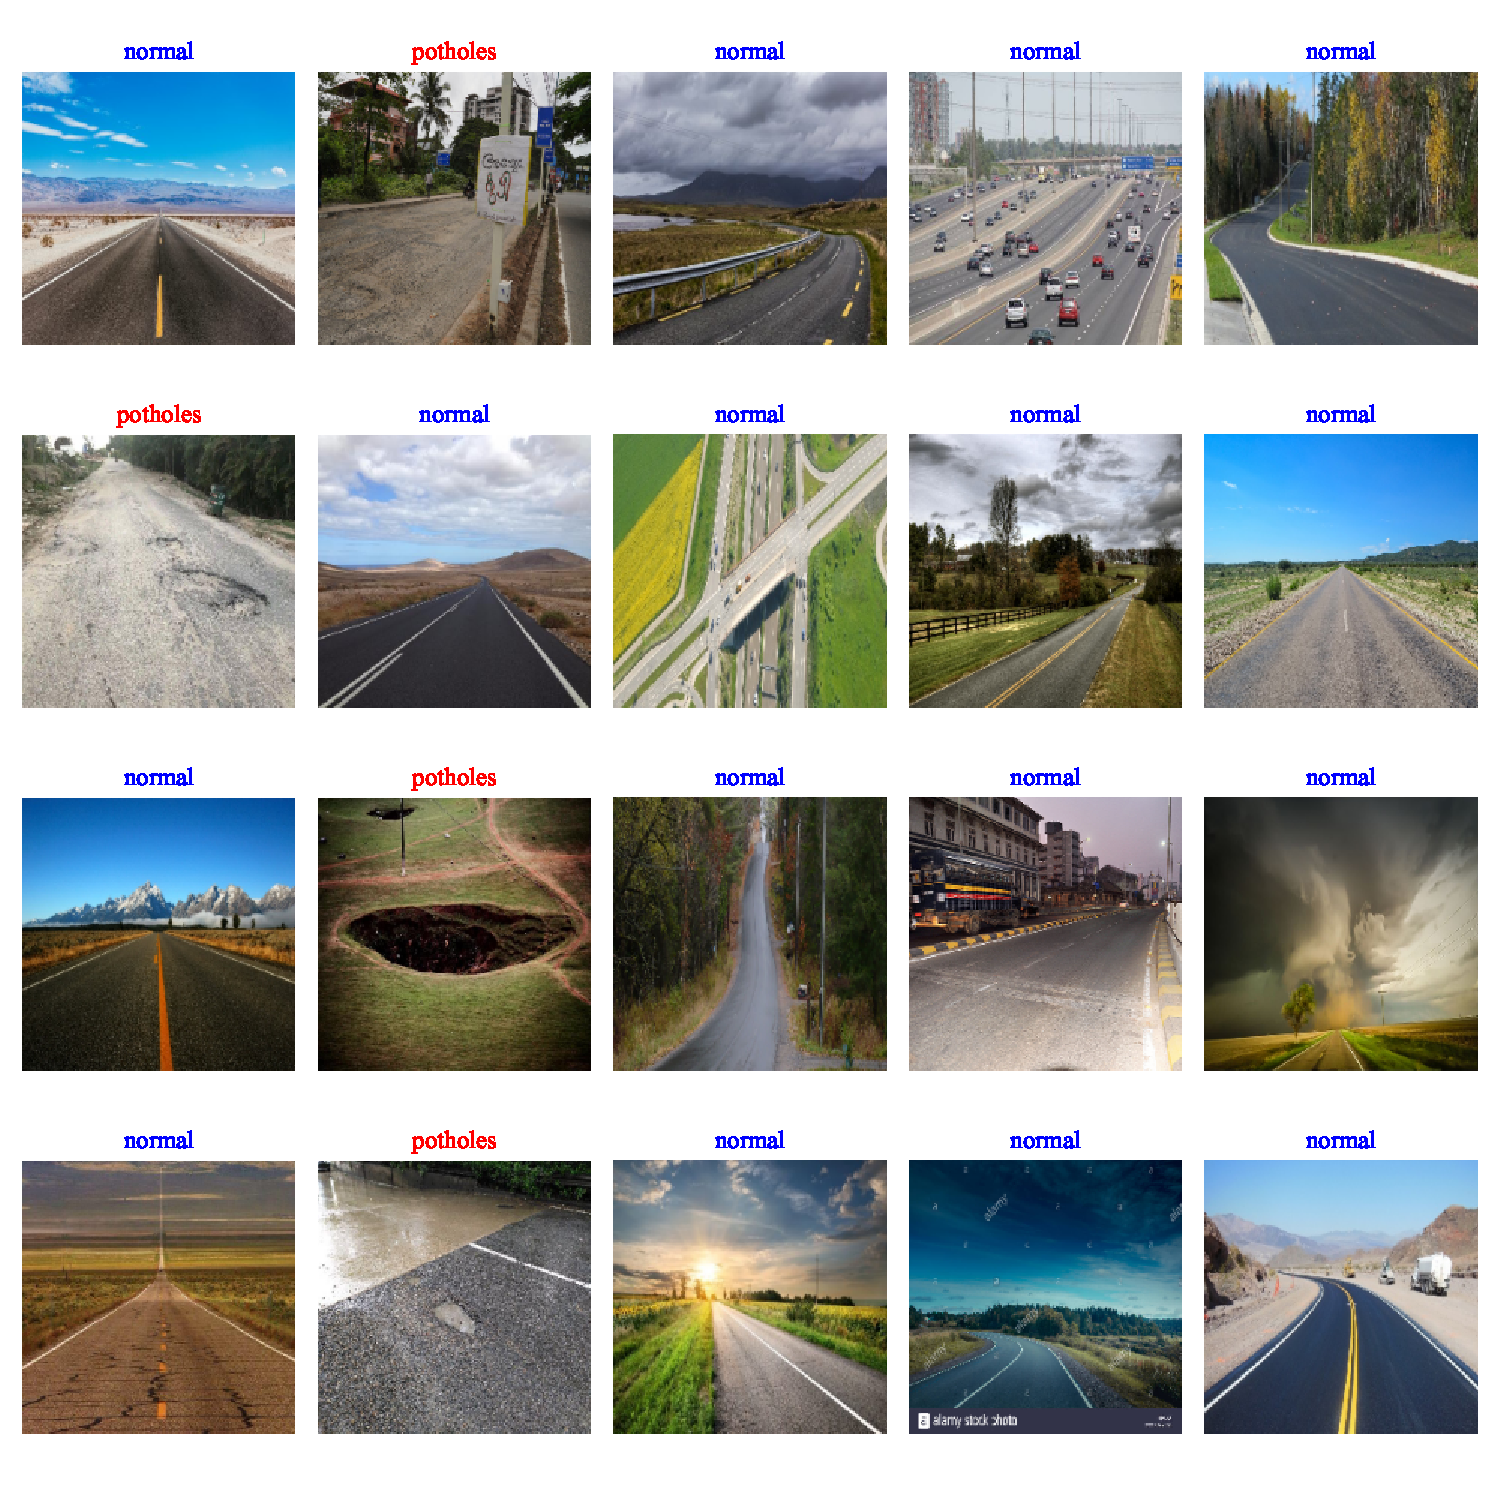
\includegraphics[scale=0.5]{图像数据观测.pdf}
		\caption{图像数据观测}
		\label{fig:图像数据观测}
	\end{figure}
	至此,我们已将所有数据进行了人为再分类,并将数据集分别放于“normal”及“potholes”文件夹中,方便后续的处理。
	\subsection{正常与坑洼道路的比较分析、图像特征提取}\label{分析}
	为了方便后续模型的分析、建立与求解,我们还需要对图像数据进行机理分析,将标记为正常及坑洼的道路进行比较分析,并提取图像的特征。因此,我们从以下几个方面进行分析:
	\begin{itemize}
		\item \textbf{原图、热力图对比}:分析坑洼与正常道路的表层区别。
		\item \textbf{RGB、灰度直方图}:分析坑洼与正常道路的图像信息分布。
		\item \textbf{边缘、轮廓检测}:分析坑洼与正常道路的边缘、轮廓特征。
		\item \textbf{阈值分割}:分析坑洼与正常道路的阈值分割特征。
	\end{itemize}
	
	但由于图片较多,故我们选择“normal133.jpg”及“potholes1.jpg”进行对比分析。以下是具体分析内容,该部分具体处理代码见\textbf{附录-C.2,Comparative Analysis of Normal and Potholes [正常与坑洼道路的比较分析]}。
	\subsubsection{原图、热力图对比}
	“normal133.jpg”及“potholes1.jpg”原图及热力图对比,如\textcolor{blue}{\cref{fig:原图对比}}及\textcolor{blue}{\cref{fig:热力图对比}}所示\textcolor{blue}{\footnote{本文所有可视化图示均为矢量图,若读者在阅读时发现图示字体过小,可适当放大 PDF页面,详细查看图示数据等。此外,本文所有图示、表格均已交叉引用,读者阅读PDF时可点击对应图表,进行跳转。}}。
	\begin{figure}[H]
		\centering
			\centering
			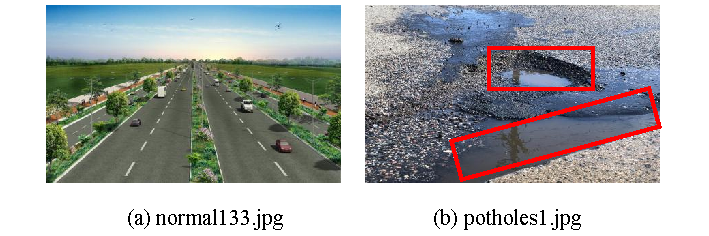
\includegraphics[scale=0.96]{[原图对比]normal133与potholes1.pdf}
			\caption{原图对比}
			\label{fig:原图对比}
	\end{figure}
	
	对比正常道路和坑洼道路的热力图,我们发现若整个道路的状况相同,没有坑洼,则那一片区域的热力值近似相同,热力图呈现的颜色相仿;若道路中的某一块状况与周围不同,如出现坑洼,则出现坑洼的区域热力值发生变化,使在热力图中呈现的颜色与周围存在差异。正常道路热力值基本一致,其热力图呈现色彩差别小,而坑洼道路中非坑洼处与坑洼处热力值相差较大,坑洼处与非坑洼处颜色相比存在较大差异。
	\begin{figure}[H]
		\centering
		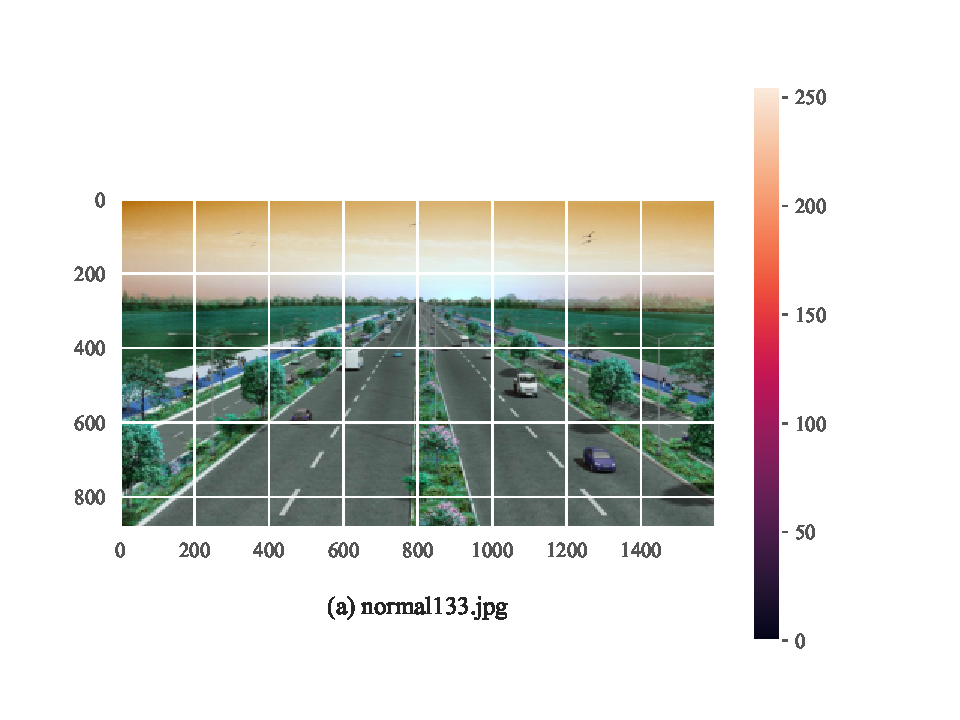
\includegraphics[scale=0.5]{normal133热力图.pdf}
		\hspace{0.3in}
		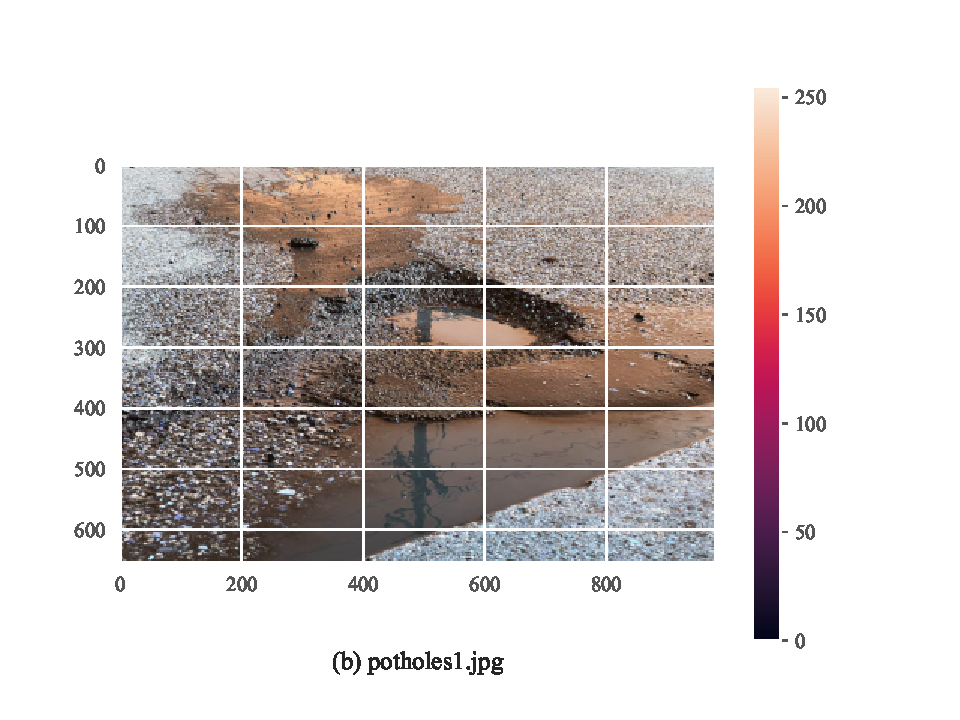
\includegraphics[scale=0.5]{potholes1热力图.pdf}
		\caption{热力图对比}
		\label{fig:热力图对比}
	\end{figure}

	\subsubsection{RGB、灰度直方图}
	“normal133.jpg”及“potholes1.jpg”RGB及灰度直方图对比,如\textcolor{blue}{\cref{fig:RGB对比}}及\textcolor{blue}{\cref{fig:灰度对比}}所示。
	
	观察RGB直方图的对比,我们可以发现两者RGB三色整体变化具有一致性,但正常道路的RGB数值整体高于坑洼道路,且正常道路RGB峰值出现在像素值为$50\text{\textasciitilde}100$之间,而坑洼道路的RGB峰值出现在像素值为$0$与$250$处。

	观察灰度直方图的对比,我们可先发现灰度直方图中正常道路所呈现的峰值远高于坑洼道路,其中坑洼道路的峰值出现在图像两侧,而正常道路的峰值出现在图像的中心位置。此外正常道路数值波动明显大于坑洼道路。故我们认为灰度直方图所展现的数值大小、分布及波动情况可以较好体现道路的坑洼情况。
	\begin{figure}[H]
		\centering
		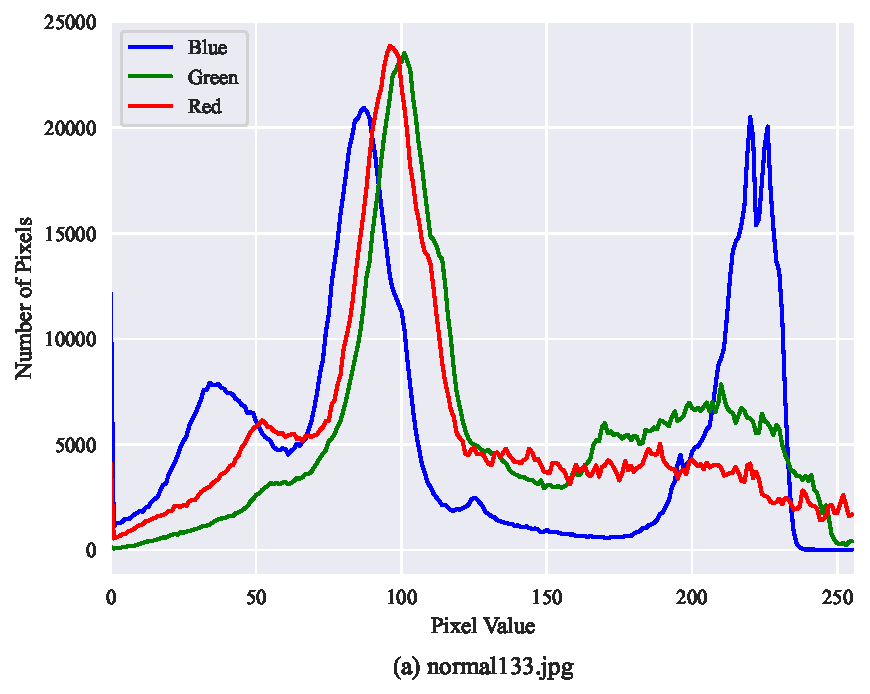
\includegraphics[scale=0.5]{normal133RGB直方图.pdf}
		\hspace{0.3in}
		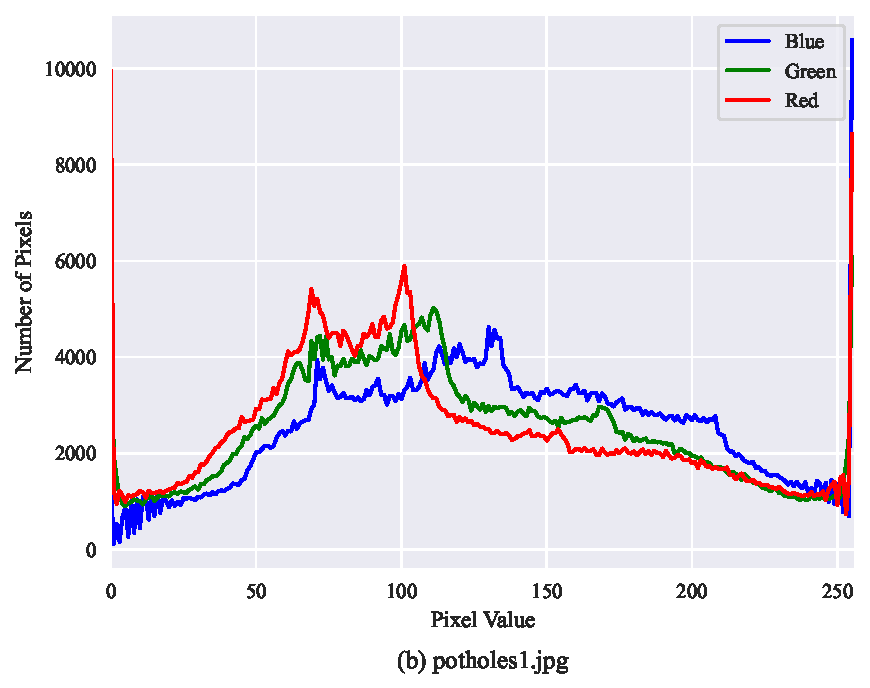
\includegraphics[scale=0.5]{potholes1RGB直方图.pdf}
		\caption{RGB直方图对比}
		\label{fig:RGB对比}
	\end{figure}
	\begin{figure}[H]
		\centering
		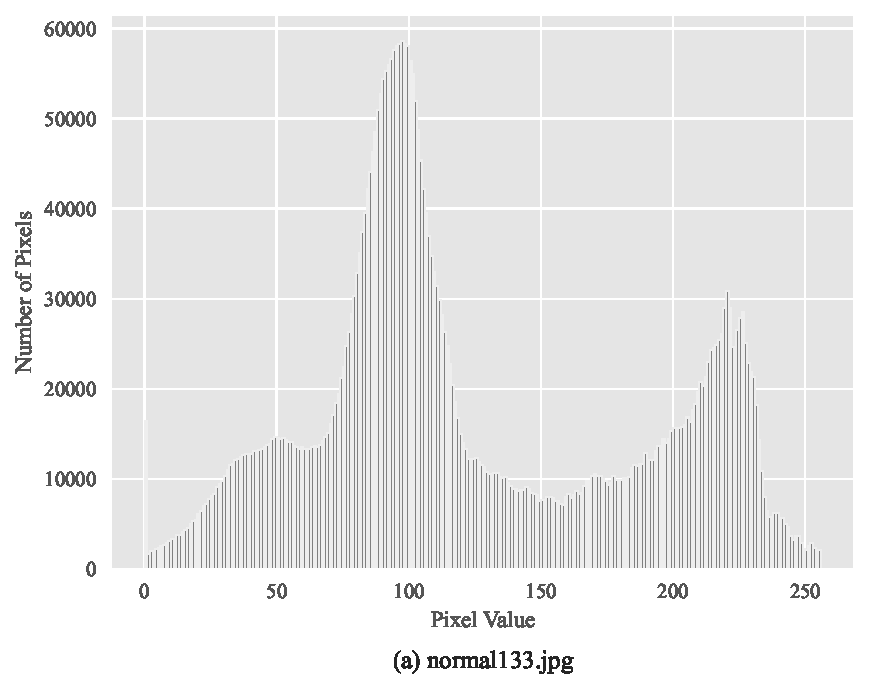
\includegraphics[scale=0.5]{normal133灰度直方图.pdf}
		\hspace{0.3in}
		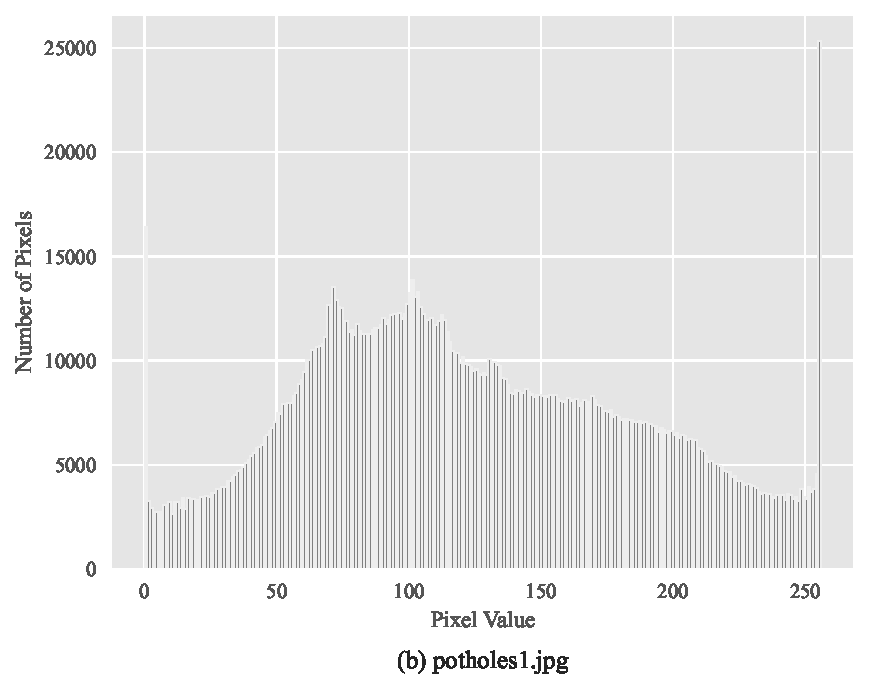
\includegraphics[scale=0.5]{potholes1灰度直方图.pdf}
		\caption{灰度直方图对比}
		\label{fig:灰度对比}
	\end{figure}
	
	\subsubsection{边缘、轮廓检测}
	“normal133.jpg”及“potholes1.jpg”边缘、轮廓检测对比,如\textcolor{blue}{\cref{fig:边缘检测}}及\textcolor{blue}{\cref{fig:轮廓检测}}所示。
	\begin{figure}[H]
		\centering
		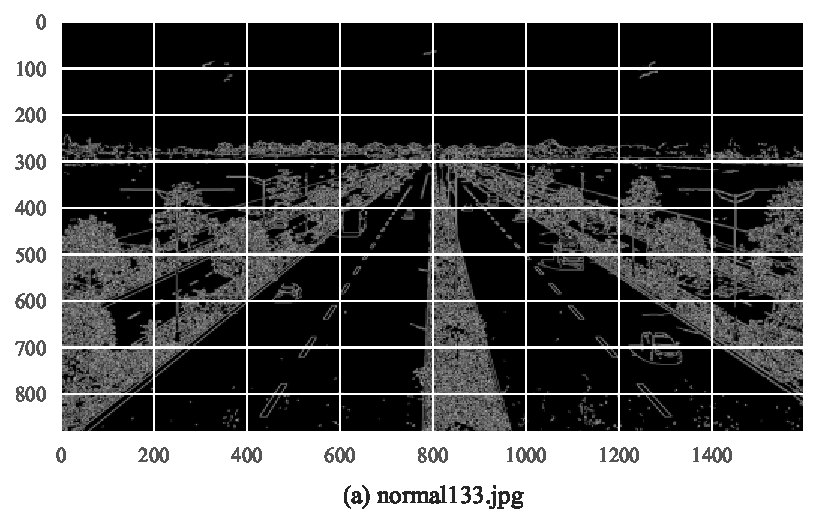
\includegraphics[scale=0.5]{normal133边缘检测.pdf}
		\hspace{0.3in}
		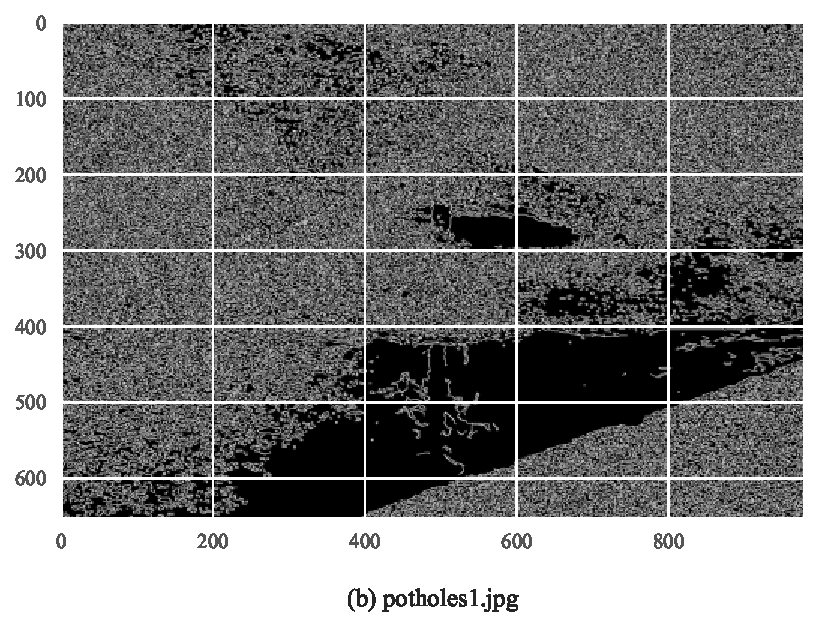
\includegraphics[scale=0.45]{potholes1边缘检测.pdf}
		\caption{边缘检测}
		\label{fig:边缘检测}
	\end{figure}
	观察边缘检测的对比,我们可以发现边缘检测后正常道路色彩连续完整,而坑洼道路的坑洼部分在边缘检测后整体呈现深度黑色,与平整的砂石路面形成了强烈对比。故我们认为采用边缘检测可以较好判断道路状况。

	对道路的图片进行轮廓检测后,我们可以发现检测后无坑洼道路的图片颜色相同,而对于坑洼道路,图片上有很明显的颜色差别。经过分析,我们认为不同的颜色代表了道路的平整与坑洼,进行轮廓检测后,可以通过道路颜色的异同判断道路是否坑洼。
	\begin{figure}[H]
		\centering
		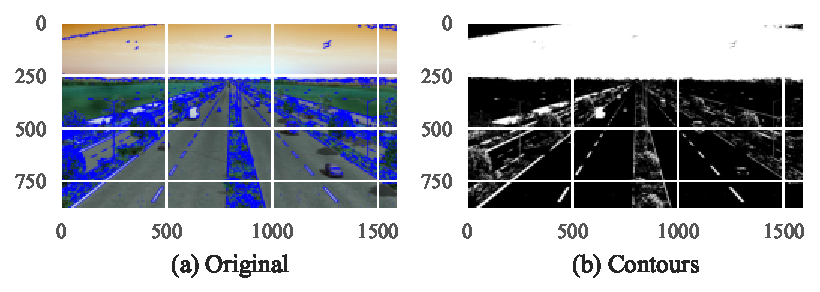
\includegraphics[scale=0.58]{normal133轮廓检测.pdf}
		\hspace{0.3in}
		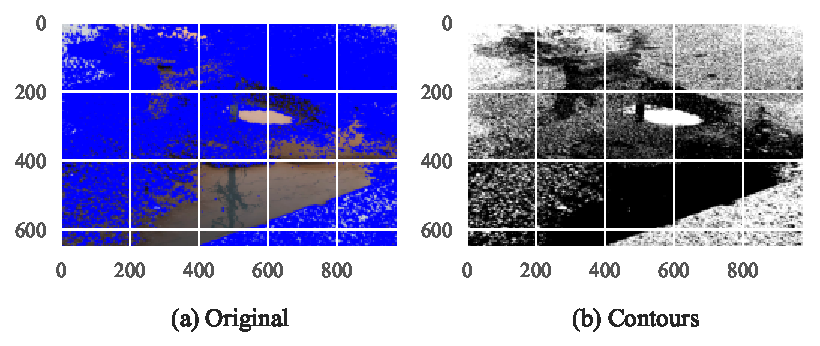
\includegraphics[scale=0.5]{potholes1轮廓检测.pdf}
		\caption{轮廓检测}
		\label{fig:轮廓检测}
	\end{figure}

	\subsubsection{阈值分割}
	“normal133.jpg”及“potholes1.jpg”阈值分割对比,如\textcolor{blue}{\cref{fig:阈值分割}}所示。
	\begin{figure}[H]
		\centering
		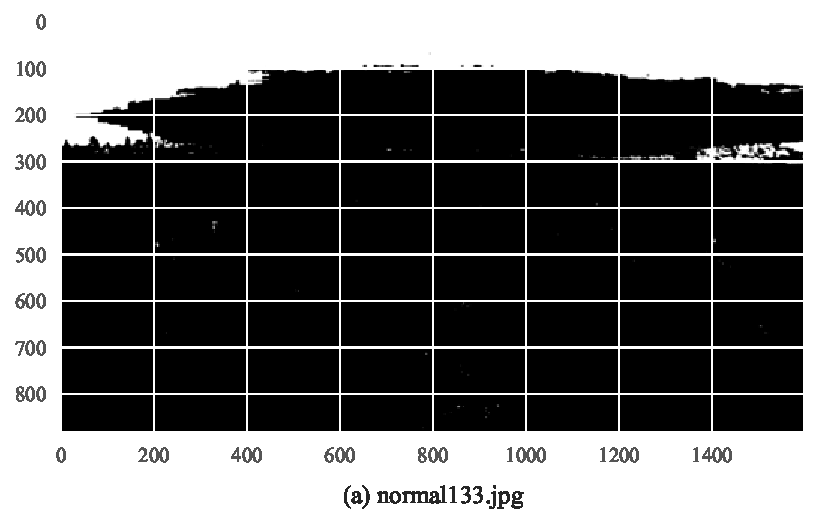
\includegraphics[scale=0.5]{normal133阈值分割.pdf}
		\hspace{0.3in}
		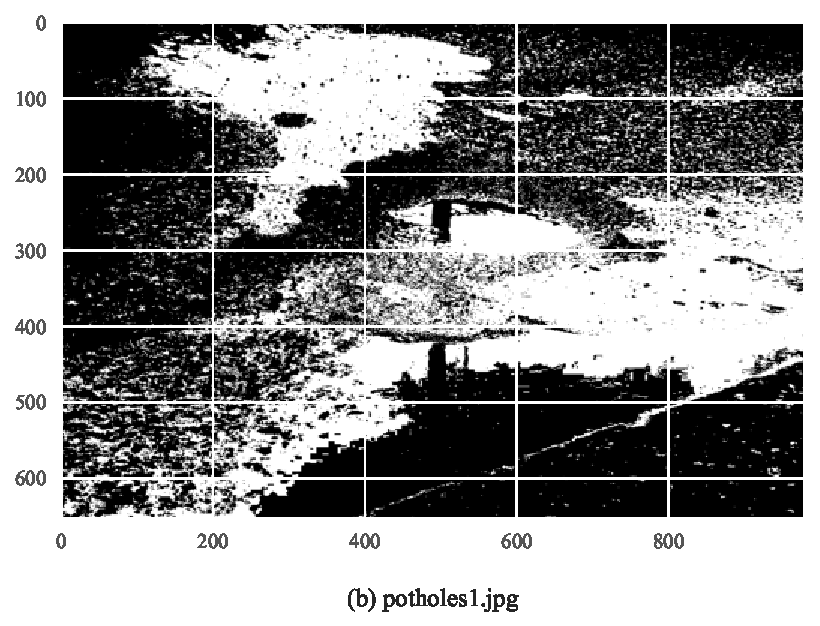
\includegraphics[scale=0.42]{potholes1阈值分割.pdf}
		\caption{阈值分割}
		\label{fig:阈值分割}
	\end{figure}
	阈值分割将图片分为两类区域,对比正常道路与坑洼道路的阈值分割图,正常道路由于整个道路的状态相同,因此经阈值分割后,全部被划分为同一类,故颜色相同;而对于坑洼道路,道路中出现了与周围状态不同的区域,经过阈值分割后,呈现出不同的颜色,黑色为正常的道路,白色为道路中存在的坑洼,色彩对比强烈。

	\subsection{图像数据预处理}
	\subsubsection{opencv读取图像文件}
	考虑到图像文件较多,为方便后续处理,我们利用Python的opencv及os库,将数据加载至内存中。并分析各类中包含的图像数据个数,如\textcolor{blue}{\cref{tab:数据信息}}所示。这里罗列了原数据集与经过\textcolor{blue}{\nameref{图像文件预处理}}部分处理后的情况,同时还计算出正常道路与坑洼道路数据个数的比值。

\begin{table}[H]
	\centering
	\caption{数据信息}
	\scalebox{0.9}{
	  \begin{tabular}{ccccc}
	  \toprule
	  \textbf{类别} & \textbf{1:正常道路} & \textbf{0:坑洼道路} & \textbf{正常道路与坑洼道路图像数据个数比值} & \textbf{合计} \\
	  \midrule
	  原数据图像个数 & 266   & 35    & 7.60  & 301 \\
	  处理后图像个数 & 259   & 41    & 6.32  & 300 \\
	  \bottomrule
	  \end{tabular}}
	\label{tab:数据信息}
\end{table}
	
	\subsubsection{图像数据两类平衡化}
	我们需要重点关注\textcolor{blue}{\cref{tab:数据信息}}中正常道路与坑洼道路数据个数的比值,发现正常道路图像个数为坑洼道路图像个数的6.32倍,这意味着正常道路图像数据的数量远大于坑洼道路图像数据的数量,即对于该二分类,其数据是不平衡的,这将会对后续模型的建立与求解造成一定的影响,易造成模型的偏向性学习。因此我们需要对现有的数据进行平衡化。即尽量使得正常道路图像数据与坑洼道路图像数据的数量相近,从而使得模型的学习均衡,减少模型的偏向性。

	该处我们采用的方法是对数据集拓充,拓充的图为原数据集中尚未出现过的图像,新图像数据来源于\url{https://www.kaggle.com/}及\url{https://github.com/}。即原数据集为新数据集的子集。具体数据见\textcolor{blue}{\cref{tab:新旧数据集}}。

\begin{table}[htbp]
	\centering
	\caption{新旧数据集信息}
	\scalebox{0.9}{
	  \begin{tabular}{ccccc}
	  \toprule
	  \textbf{数据集} & \textbf{1:normal} & \textbf{0:potholes} & \textbf{正常道路与坑洼道路图像数据个数比值} & \textbf{总计} \\
	  \midrule
	  经预处理的数据集 & 259   & 41    & 6.32  & 300 \\
	  新数据集  & 352   & 329   & 1.07  & 681 \\
	  \bottomrule
	  \end{tabular}}
	\label{tab:新旧数据集}
\end{table}
	这里,我们将随机选择10张图像进行展示,如\textcolor{blue}{\cref{fig:新旧数据集图像}}所示。
	\begin{figure}[H]
		\centering
		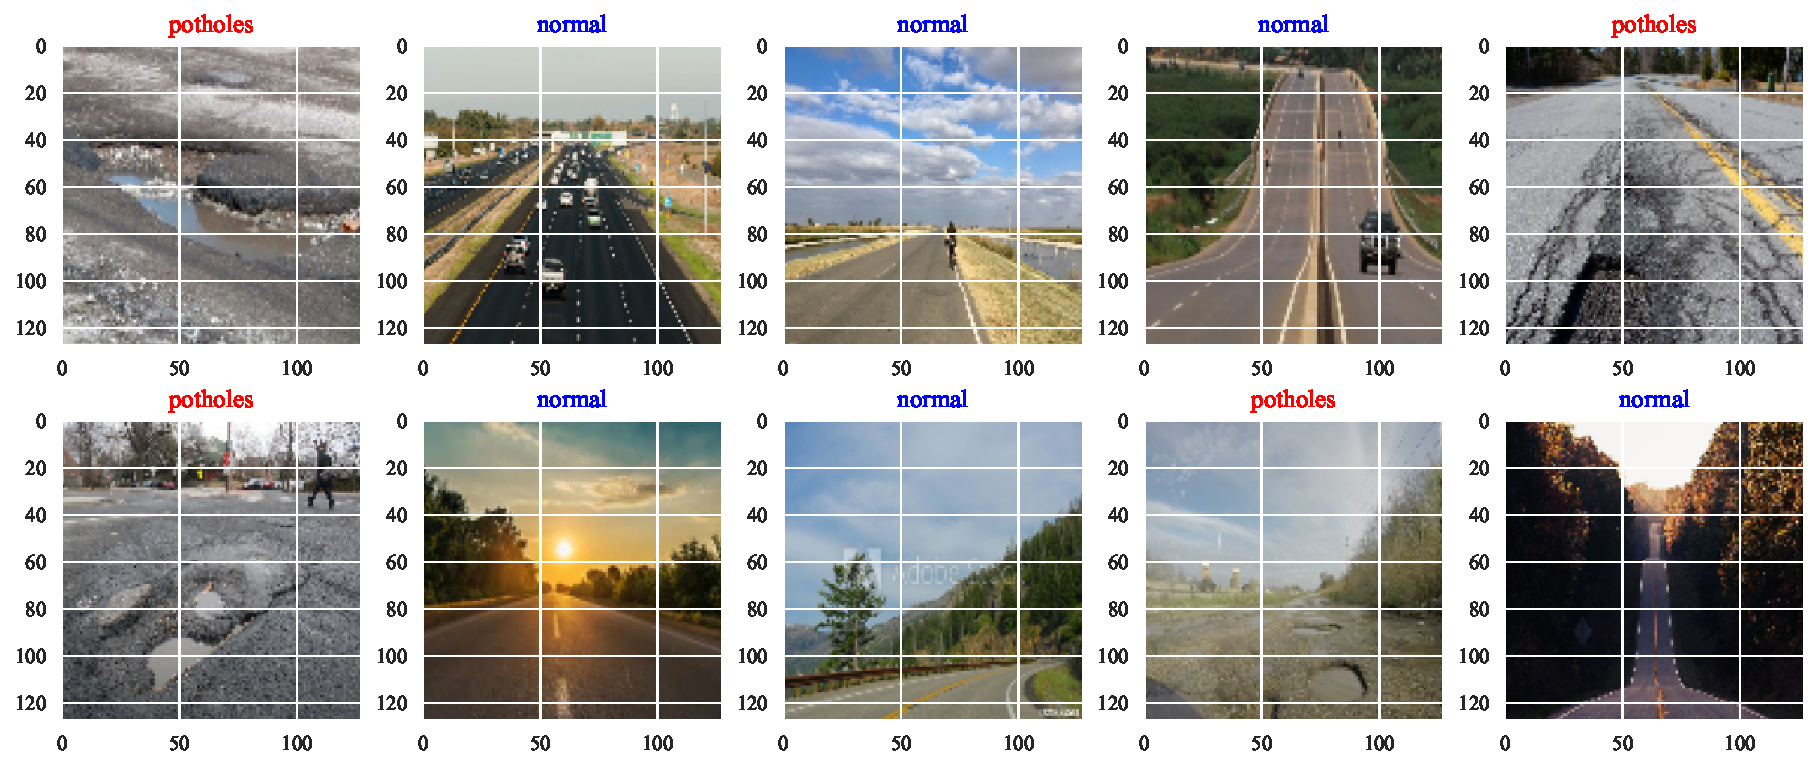
\includegraphics[scale=0.5]{CNN训练样本.pdf}
		\caption{新旧数据集图像}
		\label{fig:新旧数据集图像}
	\end{figure}
	\subsubsection{划分训练集与测试集}
	对于模型的学习,我们需要对数据集进行划分,划分为训练集与测试集。训练集用于模型的训练,测试集用于对模型性能的评估分析,检验模型效果。由于该数据集样本较少,我们设置训练集占比为$80\,\%$,测试集占比为$20\,\%$,且上述划分为采用Python的sklearn库中model\_selection.train\_test\_split方法及自定义地客观地随机划分。

	\subsubsection{训练集数据增强}
	观察数据集,发现其特征多数存在相似性;同时,数据集样本较少。因此,为避免模型的过拟合与欠拟合,这里我们需要对训练集进行数据增强\textcolor{blue}{\footnote{\textbf{注意:}这里数据增强是在划分训练集与测试集之后的,并且仅对训练集数据进行增强,并不对测试集进行划分。这是由于,若在划分训练集与测试集之前进行增强,则会造成数据泄露,影响模型的准确性,以及对未知数据的泛化能力。}}。从而增强模型对于未知数据集的泛化能力,提升模型的稳健性。

	这里,我们选用线性滤波中的\textbf{高斯滤波(Gauss Blur)}、非线性滤波中的\textbf{双边滤波(Bilateral Blur)}、以及对图像进行\textbf{顺时针旋转$\boldsymbol{\frac{\pi}{6}}$}处理。
	\begin{itemize}
		\item \textbf{高斯滤波}是一种线性平滑滤波。其基本原理是使用高斯核对图像进行卷积操作,进行加权平均的过程。每一个像素点的值,都由其邻域内的其他像素值和本身经过加权平均后得到。高斯核的标准差和大小决定了滤波器的效果,标准差越小,滤波器的效果越不明显,但是不会导致图像的细节信息丢失。其权值随着距离中心像素点的距离增加而逐渐减小,从而保留了图像的边缘信息。使用公式如下:
		\begin{equation}
			G\left(X,Y\right)=\frac{1}{2\pi\sigma^2}\exp\left(-\frac{X^2+Y^2}{2\sigma^2}\right)
		\end{equation}
		\item \textbf{双边滤波}是一种基于高斯滤波的非线性滤波方法,目的是解决高斯滤波造成的边缘模糊。结合图像的空间邻近度和像素值相似度,同时考虑空域信息和灰度相似性,实现保边去噪。双边滤波器比高斯滤波多一个高斯核。它是基于像素颜色分布的高斯滤波函数,所以在边缘附近,当两个像素距离很近时,只有同时当颜色很接近时影响才会较大,反之,虽然距离很近,但颜色差距较大,那么平滑权重也会很小。
		
		为实现双边滤波,我们首先定义滤波器的参数,即空间域核函数和像素值域核函数;然后计算出每个像素在空间域和像素值域上的权重;最后根据计算得到的权重,对每个像素的周围像素进行加权平均,以得到滤波后的像素值。其公式可表示为:
		\begin{equation}
			I_f\left( X,Y \right) =\frac{1}{G_s\left( X,Y \right)}\sum_{\left( i,j \right) \in \Omega}{I\left( X+i,Y+j \right) \cdot F_s\left( i,j \right)}\cdot F_f\left[ I\left( X,Y \right) ,I\left( X+i,Y+j \right) \right] 
		\end{equation}
		上式中各参量含义如下:
		\begin{itemize}
			\item $I_f\left(X,Y\right)$:滤波后的图像像素值;
			\item $I\left(X,Y\right)$:原始图像像素值;
			\item $G_s\left(X,Y\right)$:归一化权重;
			\item $\Omega$:滤波邻域窗口;
			\item $F_s\left(i,j\right)$:空间域核函数;
			\item $F_f\left[ I\left( X,Y \right) ,I\left( X+i,Y+j \right) \right]$:像素值域核函数。
		\end{itemize}
	\end{itemize}
\newpage
	这里,我们随机选择一张图片,将其经过上述处理后的图像一一展示,如\textcolor{blue}{\cref{fig:原图高斯双边滤波及旋转对比}}所示。经过上述处理后,在一定程度上可以增加训练集数据的多样性,从而模型可以学习到更多关于正常或坑洼道路的特征,因而有利于提升模型的泛化能力。
	\begin{figure}[H]
		\centering
		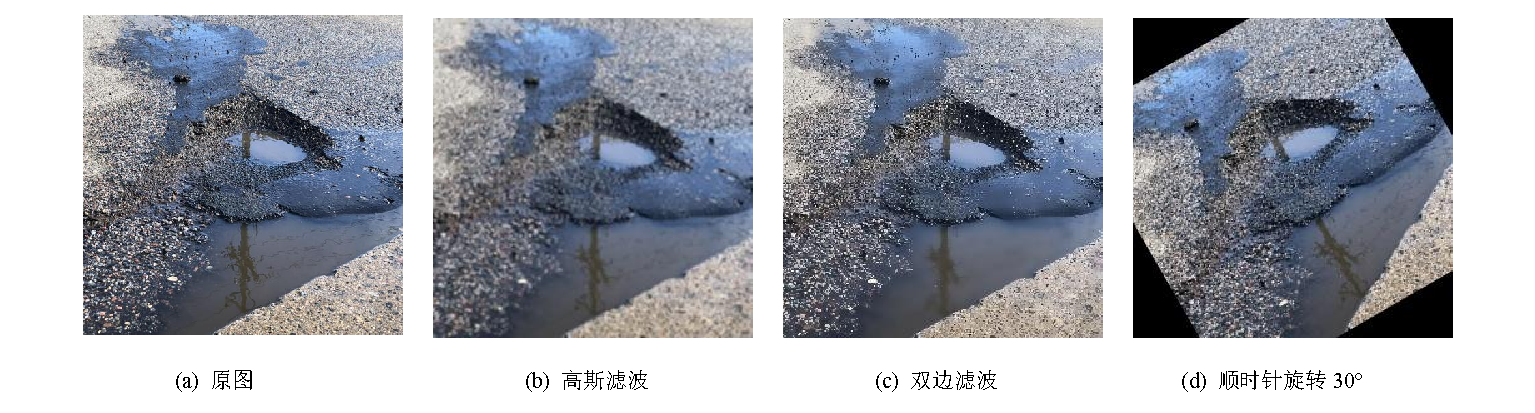
\includegraphics[scale=0.6]{原图高斯双边滤波及旋转对比.pdf}
		\caption{原图、高斯滤波、双边滤波、顺时针旋转30度}
		\label{fig:原图高斯双边滤波及旋转对比}
	\end{figure}

	经过上述滤波及旋转处理后,意味着将训练集增加3倍,即现有训练集为$681\times 0.8\times 4=2179$张图像。这里,我们将随机选择10张图像进行展示,如\textcolor{blue}{\cref{fig:数据增强}}所示。
	\begin{figure}[H]
		\centering
		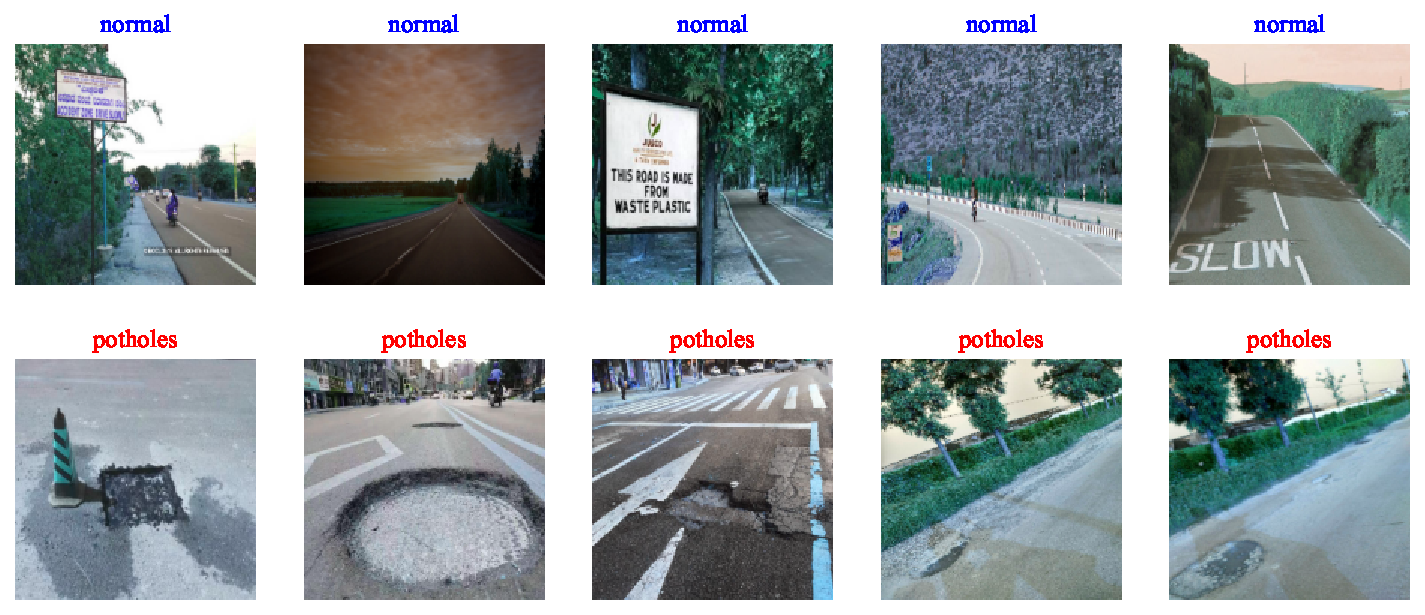
\includegraphics[scale=0.6]{PCA-SVM训练样本.pdf}
		\caption{数据增强图像}
		\label{fig:数据增强}
	\end{figure}
	\subsection{分类模型的建立}
	\subsubsection{基于主成分分析降维、网格调优的支持向量机}
	由于读取的数据本质上为特征向量,其维度较高,对于模型的训练时长、复杂度将会造成一定影响,因此这里我们首先使用\textbf{主成分分析(Principal Component Analysis, PCA)}对数据集进行降维,其实质上是将$k$维特征映射到$n$维上,这$n$维是新的正交特征,即主成分。PCA的工作就是从原始的空间中找一组相互正交的坐标轴。其中,第一个新坐标轴选取是原始数据中方差最大的方向,第二个新坐标轴选取是与第一个坐标轴正交的平面中使得方差最大的方向,第三个轴是与第一、二个轴正交的平面中方差最大的方向。以此类推,可以得到$k$个坐标轴。通过这种方式获得的新的坐标轴大部分方差都均含在上述的$n$个坐标轴中,后面的坐标轴所含的方差近似于$0$。因此,我们可以忽略之后的坐标轴,只保留前面$k$个含有绝大部分方差的坐标轴。这相当于只保留包含绝大部分方差的维度特征,而忽略包含方差几乎为$0$的特征维度,从而对数据特征的降维处理。我们通过一组数据的样本均值和样本方差计算出两个样本之间的协方差,根据所求的协方差矩阵计算其特征值与特征向量,再将特征向量单位化得到基向量变换矩阵,最后利用基向量变换矩阵与原始矩阵做内积,得到降维后的矩阵。对数据集计算协方差矩阵,公式如下:
	\begin{equation}
		\boldsymbol{C}=\left[ \begin{matrix}
			\text{Cov}\left( X_1,X_2 \right)&		\text{Cov}\left( X_1,X_2 \right)&		\cdots&		\text{Cov}\left( X_1,X_n \right)\\
			\text{Cov}\left( X_2,X_1 \right)&		\text{Cov}\left( X_2,X_2 \right)&		\cdots&		\text{Cov}\left( X_2,X_n \right)\\
			\vdots&		\vdots&		\ddots&		\vdots\\
			\text{Cov}\left( X_n,X_1 \right)&		\text{Cov}\left( X_n,X_2 \right)&		\cdots&		\text{Cov}\left( X_n,X_n \right)\\
		\end{matrix} \right] \label{C}
	\end{equation}
	其中,每一个元素定义如下\textcolor{blue}{\cite{刘建新}}:
	\begin{equation}
		\text{Cov}=\left( X,Y \right)=E\left\{\left[X-E\left(X\right)\right]\left[Y-E\left(X\right)\right]\right\}=E\left(XY\right)-E\left(X\right)E\left(Y\right) \label{Cov}
	\end{equation}
	其中$E\left(X\right)$为该列数据的均值。

	之后,计算上述协方差矩阵的特征值$\lambda_n$及其对应的特征向量$\boldsymbol{u}_{nj}$,这里我们不妨令$\lambda_1\geqslant\lambda_2\geqslant\cdots\lambda_n\geqslant 0$,由特征向量组成$n$和新的指标变量
	\begin{equation}
		\left\{ \begin{array}{l}
			y_1=\boldsymbol{u}_{11}x_1+\boldsymbol{u}_{21}x_2+\cdots +\boldsymbol{u}_{n1}x_n\\
			y_2=\boldsymbol{u}_{12}x_1+\boldsymbol{u}_{22}x_2+\cdots +\boldsymbol{u}_{n2}x_n\\
			\vdots\\
			y_3=\boldsymbol{u}_{1n}x_1+\boldsymbol{u}_{2n}x_2+\cdots +\boldsymbol{u}_{nn}x_n\\
		\end{array} \right. 
	\end{equation}
	其中$y_n$是第$n$个主成分。

	在PCA的基础上,我们建立\textbf{支持向量机(Support Vector Machine, SVM)}二分类模型。其是建立在结构风险最小原理及Vapnik-Chervonenkis理论基础之上的\textcolor{blue}{\cite{汪海燕}},以有限的数据信息,在数据样本中找出合适区分类别的决策分界面,与合适的边界分界面。实现分类误差最小的问题实质即求解下列方程\textcolor{blue}{\cite{张松兰}}:
	\begin{equation}
		\begin{array}{cl}
			\min & L\left( \omega \right) =\frac{1}{2}\lVert \omega \rVert +C\sum\limits_{i=1}^n{\xi}\\
			\text{s.t.\ } & y_i\left( \omega ^{\text{T}}\varphi \left( x_i \right) +b \right) \geqslant 1-\xi\\
		\end{array}
	\end{equation}
	其中,$\xi>0$为松弛变量,$\varphi\left(x_i\right)$为核函数,$C$为惩罚系数。

	此外,可针对不同的数据集的特征选择不同的\textbf{核函数(Kernel Function)},从而达到较优秀的效果。对于该数据集,我们选择\textbf{高斯核函数(Radial Basis Function,RBF)},其定义公式如下:
	\begin{equation}
		K\left(x_i, x_j\right)=\exp \left(-\frac{\left\|x_i-x_j\right\|^{2}}{2\sigma^{2}}\right)=\exp \left(-\gamma \left\|x_i-x_j\right\|^{2}\right)
	\end{equation}
	
	同时,为了将模型效果优化,我们将对SVM模型的超参数进行调优。这里我们选用\textbf{网格调优(Grid Search)},对惩罚系数$C$进行调优,最终选定的$C=1.90$。具体实现代码见\textbf{附录-C.4  PCA-SVM [PCA降维、网格调优的支持向量机]}。

	\subsubsection{深度学习:CNN卷积神经网络}
	卷积神经网络是一类包含卷积计算且具有深度结构的前馈神经网络。\textbf{它主要由输入层、卷积层、激活层、池化层和全连接层构成}\textcolor{blue}{\cite{李莎}}。其具体框架如\textcolor{blue}{\cref{fig:CNN原理图}}所示。
	\begin{figure}[H]
		\centering
		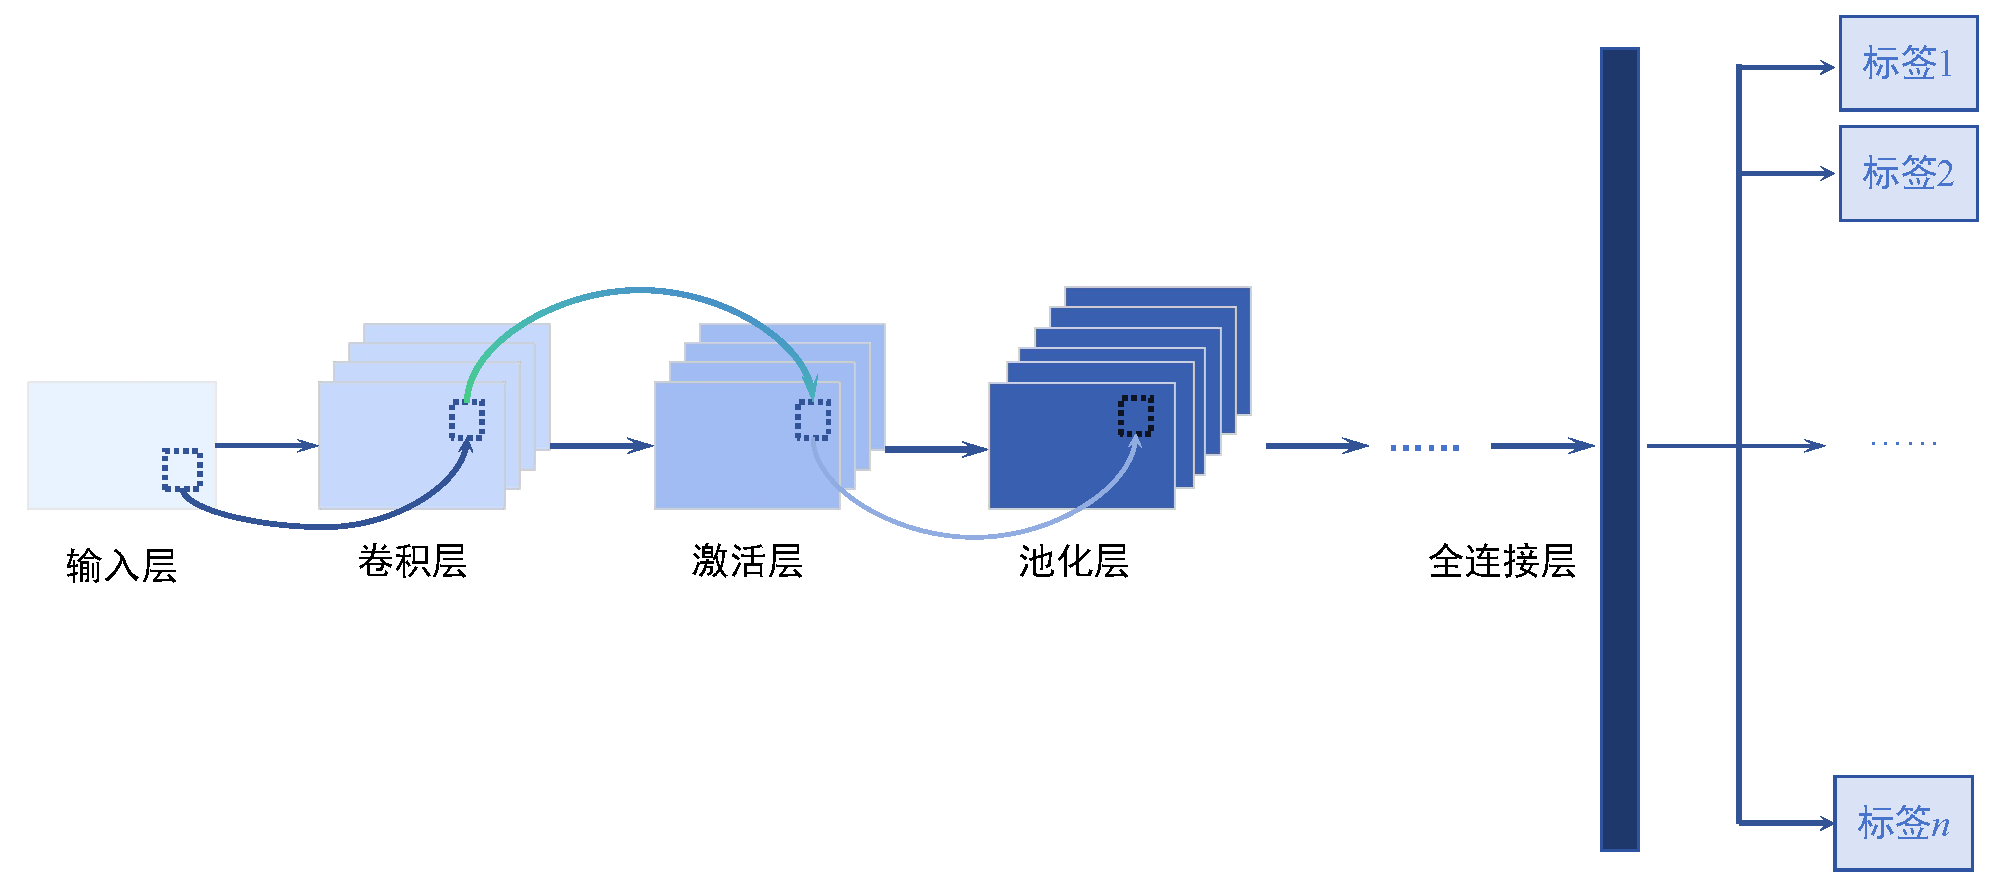
\includegraphics[scale=0.36]{CNN原理图.pdf}
		\caption{CNN原理图}
		\label{fig:CNN原理图}
	\end{figure}

	其首先于输入层对数据进行去均值处理,而后在卷积层进行特征提取,将特征通过激活函数映射到数学空间形成特征图并将输出结果于激活层进行非线性映射\textcolor{blue}{\cite{孟琪琳}},接着在池化层中将特征降维压缩,降低复杂程度。池化的常见方法有平均池化和最大池化两种,最大池化是将输入图像分割为多个子区域,然后从每个子区域中选择最大像素值作为子区域的输出值,以此对输入图像的尺寸和特征进行采样和减少,以减少计算量。平均池化是将输入图像分割为多个子区域后计算每个子区域所有像素值的平均值,将平均值作为子图像的输出值,也可以减少计算量\textcolor{blue}{\cite{刘幸倩}}。最后传递至全连接层,将全连接层各节点与上一层所有的节点结合起来。平均池化计算公式及最大池化计算公式为:
	\begin{equation}
		p_{l}^{\left( i,j \right)}=\frac{1}{S}\sum_{x=id}^{id+d}{\sum_{y=jd}^{jd+d}{a_{l}^{\left( x,y \right)}}}
	\end{equation}
	最大池化计算公式为:
	\begin{equation}
		p_{l}^{\left( i,j \right)}=\underset{\left( id,jd \right) \leqslant \left( x,y \right) \leqslant \left( id+d,jd+d \right)}{\max}a_{l}^{\left( x,y \right)}
	\end{equation}
	其中,$p_{l}^{\left( i,j \right)}$为第一层中坐标为$p_{l}^{\left( i,j \right)}$的特征值,$S$为池化区域的面积,$a_{l}^{\left( x,y \right)}$为输入特征图中坐标为$\left( x,y \right)$的特征值,$d$为步长。

	\begin{equation}
		p_{l}^{\left( i,j \right)}=\frac{1}{S}\sum_{x=id}^{id+d}{\sum_{y=jd}^{jd+d}{a_{l}^{\left( x,y \right)}}}
	\end{equation}

	根据\textcolor{blue}{\nameref{分析}}部分的分析,对于该分类问题及数据集的特征,我们对CNN卷积神经网络的结构进行架构,具体如下:
	\begin{itemize}
		\item \textbf{卷积层:}输入形状为$128\times 128$像素,$3$个通道(RGB图像),$32$个卷积核,卷积核大小为$5\times 5$,激活函数为ReLU
		\item \textbf{最大池化层:}池化窗口大小为$2\times 2$
		\item \textbf{卷积层:}输入形状为$64$个通道,卷积核大小为$3\times 3$,激活函数为ReLU
		\item \textbf{最大池化层:}池化窗口大小为$2\times 2$
		\item \textbf{卷积层:}输入形状为$128$个通道,卷积核大小为$3\times 3$,激活函数为ReLU
		\item \textbf{最大池化层:}池化窗口大小为$2\times 2$
		\item \textbf{卷积层:}输入形状为$128$个通道,卷积核大小为$3\times 3$,激活函数为ReLU
		\item \textbf{最大池化层:}池化窗口大小为$2\times 2$
		\item \textbf{卷积层:}输入形状为$128$个通道,卷积核大小为$3\times 3$,激活函数为ReLU
		\item \textbf{最大池化层:}池化窗口大小为$2\times 2$
		\item \textbf{展平层:}将卷积层的输出展平为一维数组
		\item \textbf{随机丢弃层:}丢弃比例为$40\,\%$
		\item \textbf{全连接层:}输入为展平后的数据,$128$个神经元,激活函数为ReLU
		\item \textbf{全连接层:}输入为$128$个神经元,输出为$2$个类别(类别标签为$0$和$1$),激活函数为softmax
	\end{itemize}
	
	为更好地展现CNN模型的架构,我们将其可视化,如\textcolor{blue}{\cref{fig:CNN模型架构}}所示。具体处理代码见\textbf{附录-C.5,CNN [卷积神经网络]}。
	\begin{figure}[H]
		\centering
		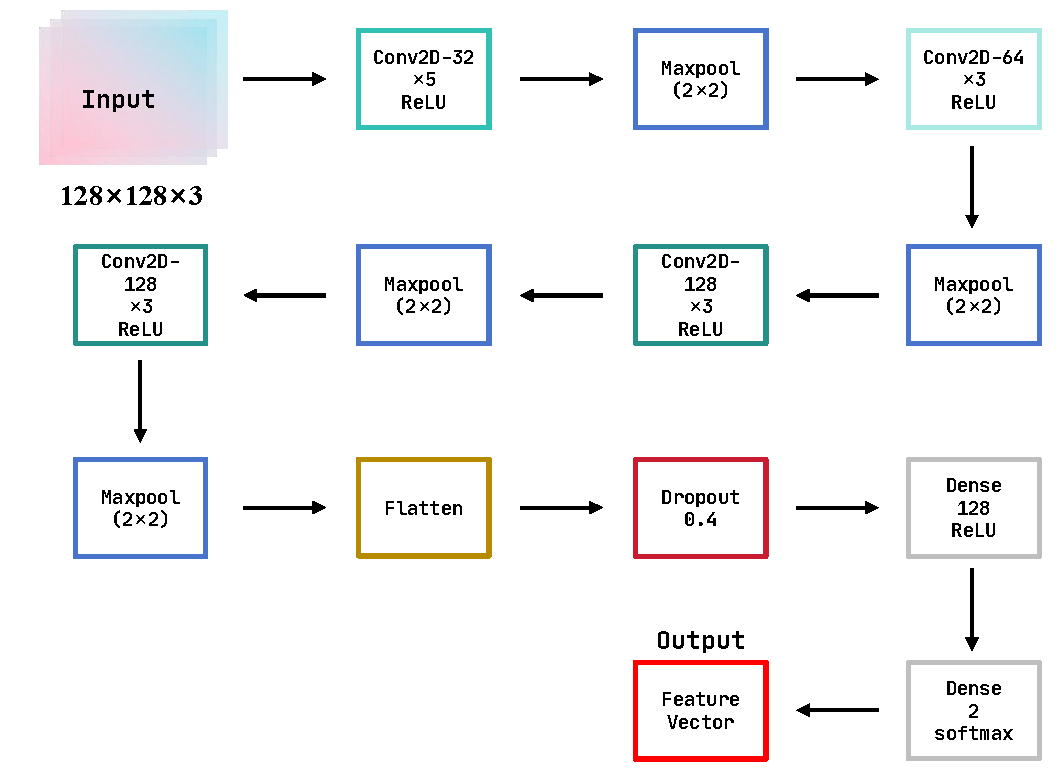
\includegraphics[scale=0.66]{CNN架构.pdf}
		\caption{CNN模型架构}
		\label{fig:CNN模型架构}
	\end{figure}
	\subsubsection{CNN-SVM的分类模型}
	传统的CNN模型由输入层、卷积层、激活层、池化层、全连接层构成,通过softmax进行输出。然而,由于softmax在针对非线性且稀疏的数据矩阵时,其效果不如传统机器学习算法\textcolor{blue}{\cite{ZHANGP}}。针对这一现象及避免单一模型的局限性,我们建立基于CNN与SVM组合的CNN-SVM模型,该模型利用基于监督学习的SVM模型实现分类,CNN模型实现特征提取。除此之外,此模型相比于传统CNN模型还增加了注意力机制\textcolor{blue}{\cite{李毅泉}},此机制可理解为将更多的权重赋值在对图像识别有影响的特征上,同时减少对图像识别意义特征较小的权重。对于该模型:其一,将传统的CNN模型的softmax归一化函数更换为SVM模型,在一定程度上能够提升模型的泛化能力\textcolor{blue}{\cite{何铠}};其二,该模型还增加了注意力机制,能够更好地提取图像信息的特征,从而提升模型精度。具体处理代码见\textbf{附录-C.6,CNN-SVM [卷积神经网络与支持向量机]}。

	\subsection{模型的评估}
	为更好地评估模型,我们针对上述三种模型进行多维度评估,并针对各模型进行针对性分析。这里我们用到的有:
	\begin{itemize}
		\item \textbf{模型训练及预测时间和($T$)}
		\item \textbf{准确率(Accuracy)}:即预测正确数占总数的比例,其计算公式如下:
			\begin{equation}
				\mathrm{Accuracy}=\frac{N_{\mathrm{TruePredict}}}{N_{\mathrm{Predict}}} \label{Accuracy}
				\end{equation}
			其中,$N_{\mathrm{TruePredict}}$为预测正确的样本数,$N_{\mathrm{Predict}}$为被预测的样本总数;
		\item \textbf{损失值(Loss)}:这里我们采用Categorical Crossentropy\textcolor{blue}{\cite{损失函数}},即交叉熵损失函数,其使用交叉熵(Cross Entropy)作为度量分类任务的差异,从而来衡量两者之间的概率分布的相似性,其公式如下:
			\begin{equation}
				\text{Loss}=-\sum_{i=1}^{\text{output size}}y_i\cdot\log\left(\hat{y}_i\right)
			\end{equation}
			其中,$y_i$为真实标签,$\hat{y}_i$为预测标签;
		\item \textbf{分类报告(Classification Report)}:其可以直观得到模型各项参数,包括每一类别的精确率(Precision),召回率(Recall),F1分数值(F1-Score)。对于这三项值,其计算公式如下:
		\begin{itemize}
			\item {\heiti 精确率}
			\begin{equation}
				\mathrm{Precision} = \frac{TP}{TP+FP} \label{Precision}
			\end{equation}
			\item {\heiti 召回率}
			\begin{equation}
				\mathrm{Recall} = \frac{TP}{TP+FN} \label{Recall}
			\end{equation}
			\item {\heiti F1分数值} 
			\begin{equation}
				\mathrm{F}1 = \frac{2\times \mathrm{Precision}\times \mathrm{Recall}}{\mathrm{Precision}+\mathrm{Recall}}=\frac{TP}{TP+\frac{1}{2}\left(FP+FN\right)} \label{F1-Score}
			\end{equation}
		\end{itemize}
		此外,对于模型的精确率、召回率,我们可以根据定义可以发现若这两项值较大,则模型效果较好。同时根据定义,我们可以发现模型的精确率、召回率在理想情况下是相差较小的,我们可以根据图示结果验证,符合预期效果。对于模型的F1分数值,其为精确率与召回率的调和平均数\textcolor{blue}{\cite{模型评测}},因此当精确率与召回率均有较好表现时,F1分数值会有较优秀表现。我们也可对\textcolor{blue}{\eqref{F1-Score}}进行一定变换,可以得到:
		\begin{equation}
			\mathrm{F}1=\frac{2}{\dfrac{1}{\mathrm{Precision}}+\dfrac{1}{\mathrm{Recall}}} \label{ReacllNew}
		\end{equation}
		根据该式,我们可以得出上述结论。

		\item \textbf{混淆矩阵(Confusion Matrix)}:矩阵每一行表示样本标签的实际类别,在本题中表示道路类型:为正常还是坑洼的实际标签;每一列表示样本标签的预测类别,在本题中表示道路类型:为正常还是坑洼的预测标签。因此该图示的主对角线数据之和即为模型预测准确的样本数。这里此外还需要引入四项值,分别为$TP$、$FN$、$FP$、$TN$,其中T为True,F为False,这两个字母表示预测值与实际值是否相同;P为Positive,N为Negative,这两个字母表示预测出的是属于正类还是负类。而混淆矩阵可以直观地观察到预测准确与错误的情况,以及模型对于每一类别的区分程度。
		\item \textbf{特征曲线及曲线下面积曲线(Receiver Operating Characteristic/Area Under the Curve, ROC/AUC)}:首先我们需要引出模型的相关参数,定义如下:
		\begin{itemize}
			\item {\heiti 灵敏度}\textbf{(Sensitivity)}。灵敏度又被称为真阳性率,即$TP$率:
			\begin{equation}
				\mathrm{Sensitivity}=TPR=\frac{TP}{TP+FN} \label{Sensitivity}
			\end{equation}
			\item {\heiti 特异性}\textbf{(Specificity)}。特异性又被称为真阴性率,即$TN$率:
			\begin{equation}
				\mathrm{Specificity}=TNR=\frac{TN}{TN+FP} \label{Specificity}
			\end{equation}
			\item \textbf{1-Specificity}。称为假阳性率(False Positive Rate, $FPR$):
			\begin{equation}
				FPR=1-\mathrm{Specificity}=\frac{FP}{FP+TN} \label{FPR}
			\end{equation}
			\item \textbf{1-Sensitivity}。称为假阴性率(False Negative Rate, $FNR$):
			\begin{equation}
				FNR=1-\mathrm{Sensitivity}=\frac{FN}{FN+TP} \label{FNR}
			\end{equation}
		\end{itemize}
		$FPR$和$FNR$均对数据分布的变化不敏感\textcolor{blue}{\cite{Tharwat}},因此这两个指标可以用于在不平衡的数据上建立的模型效果的评价。
		
		对于ROC/AUC曲线,其以每一类别的$1-\mathrm{Specificity}$即$FPR$为横坐标,以$\mathrm{Sensitivity}$即$TPR$为纵坐标,其可体现出模型的灵敏度与特异性之间的关系与差异。因此,该图的理想点位于左上角,即$FPR=0$且$TPR=1$。换言之,当曲线越靠近左上角,模型效果就越优。从而,我们可以得到另一项指标,即曲线下面积(Area Under the Curve, AUC),由上述分析可知,AUC值越高,模型的整体效果也就越优。
		\item \textbf{精确率-召回率曲线(Precision-Recall Curve)}:该图像可表现出分类的预测精度与召回率之间的关系\textcolor{blue}{\cite{Yellowbrick}}。对于预测精度与召回率的计算方式在“问题三”中已经叙述。因此图像的填充区域越大,分类效果越优。
		\item \textbf{交叉验证(Cross Validation)}:在该方法中,每一条数据用于训练的次数均相同,且恰好被检验一次。假设使用$k(k=2,3,4,\cdots)$折交叉验证,将数据分为大小相等的$k$份,在每一次学习时,选择其中一份作为检验集,而余下的数据作为训练集,上述过程重复$k$次。此外,检验集是互斥的,并且能够有效地覆盖数据集\textcolor{blue}{\cite{数据挖掘导论}}。
	\end{itemize}

	\subsubsection{三种模型的效果逐一分析}\label{模型效果}
	\begin{itemize}
		\item \textbf{PCA-SVM}

		通过查看Jupyter的代码执行记录:PCA模型在训练集训练耗时$50\,\text{s}+281\,\text{ms}$,在测试集适应耗时$2\,\text{s}+968\,\text{ms}$;SVM模型网格调优耗时$9\,\text{s}+948\,\text{ms}$,在训练集训练及在测试集测试共耗时$185\,\text{ms}$。通过在测试集的测试,经计算,该模型准确率为:$86.67\,\%$。此外,我们还得出其分类报告表,如\textcolor{blue}{\cref{tab:PCA-SVM分类报告表}}所示。
\begin{table}[htbp]
	\centering
	\caption{PCA-SVM分类报告表}
	\scalebox{0.9}{
	  \begin{tabular}{ccccc}
	  \toprule
	  \textbf{维度} & \textbf{precision} & \textbf{recall} & \textbf{f1-score} & \textbf{support} \\
	  \midrule
	  0:potholes & 0.50  & 0.25  & 0.33  & 8 \\
	  1:normal & 0.89  & 0.96  & 0.93  & 52 \\
	  accuracy &       &       & 0.87  & 60 \\
	  marco avg & 0.70  & 0.61  & 0.63  & 60 \\
	  weighted avg & 0.84  & 0.87  & 0.85  & 60 \\
	  \bottomrule
	  \end{tabular}}
	\label{tab:PCA-SVM分类报告表}
\end{table}
	观察上表,我们可以发现由于该模型尚未采用采样方法扩充数据集,虽然整体准确率较高,但对于各类别有明显的不平衡性。此外,该模型对于坑洼类别的精确率、召回率、F1分数值均较低,即说明该模型效果较为一般。
		\item \textbf{CNN}
		
		通过查看Jupyter的代码执行记录:CNN模型在训练集训练$50$轮耗时$5\,\text{m}+26\,\text{s}+888\,\text{ms}$,在测试集测试耗时$435\,\text{ms}$。通过在测试集的测试,经计算,该模型准确率为:$88.97\,\%$。此外,我们还得出其分类报告表,如\textcolor{blue}{\cref{tab:CNN分类报告表}}所示。
\begin{table}[htbp]
	\centering
	\caption{CNN分类报告表}
	\scalebox{0.9}{
	  \begin{tabular}{ccccc}
	  \toprule
	  \textbf{维度} & \textbf{precision} & \textbf{recall} & \textbf{f1-score} & \textbf{support} \\
	  \midrule
	  0:potholes & 0.90  & 0.88  & 0.89  & 68 \\
	  1:normal & 0.88  & 0.90  & 0.89  & 68 \\
	  accuracy &       &       & 0.89  & 136 \\
	  marco avg & 0.89  & 0.89  & 0.89  & 136 \\
	  weighted avg & 0.89  & 0.89  & 0.89  & 136 \\
	  \bottomrule
	  \end{tabular}}
	\label{tab:CNN分类报告表}
\end{table}

	观察该表,我们可以发现,该模型在新数据集上表现效果较优秀,各项指标均较为理想。此外,我们还绘制其在训练过程中在训练集及测试集上的准确率与损失值,如\textcolor{blue}{\cref{fig:CNN训练结果}}所示。通过观察该图,我们可以发现,随着迭代次数的增加,训练集上的准确率平稳而缓慢增加,测试集上的准确度经过起伏后也为上升趋势。而随着迭代次数增加,其训练集上的损失逐渐减少,而在测试集上其损失呈波动性,这可能是由于数据集过少,即缺乏代表性样本\textcolor{blue}{\cite{数据挖掘导论}},易造成过拟合。

	\begin{figure}[H]
		\centering
		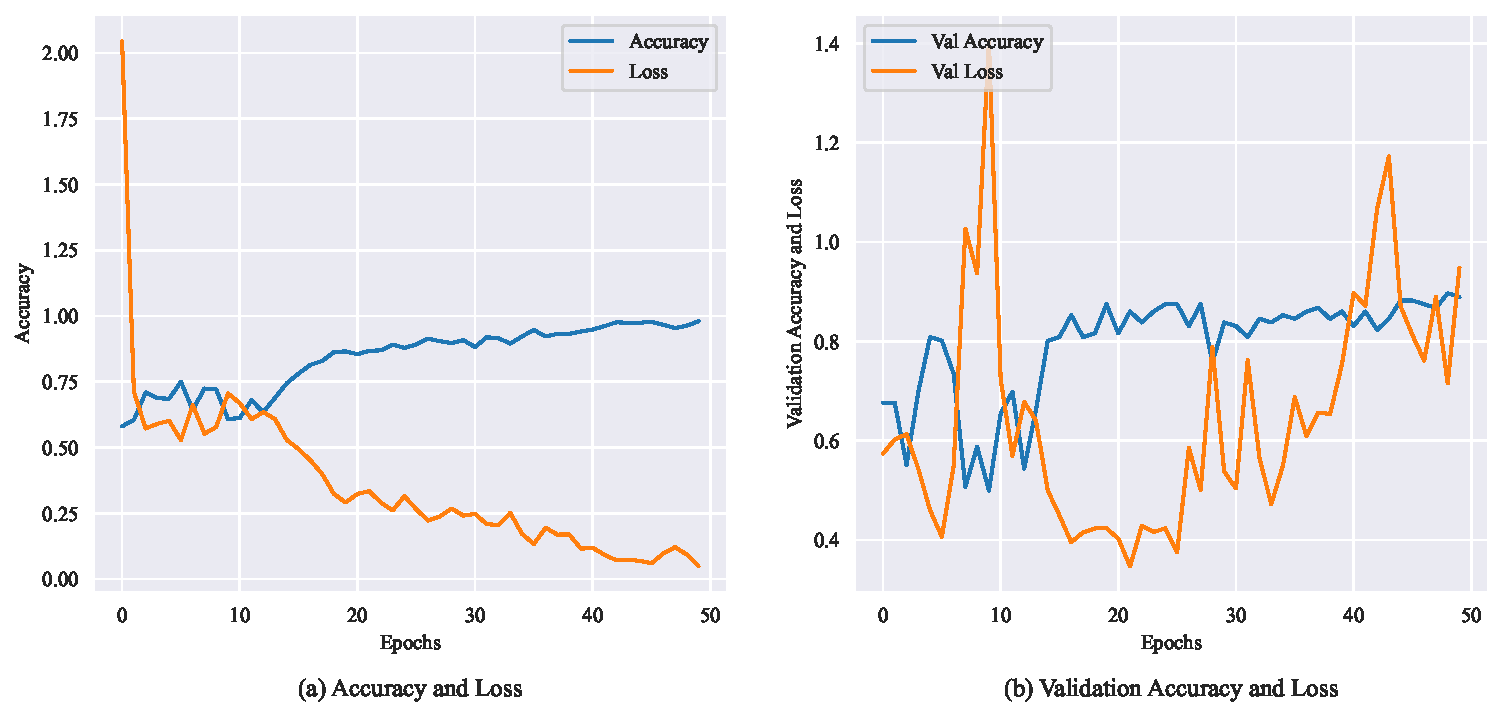
\includegraphics[scale=0.65]{CNN训练结果.pdf}
		\caption{CNN训练结果}
		\label{fig:CNN训练结果}
	\end{figure}
		\item \textbf{CNN-SVM}
		
		CNN模型训练耗时$5\,\text{m}+26\,\text{s}+888\,\text{ms}$,提取图像特征耗时$482\,\text{ms}$;SVM分类器在所提取的特征上训练耗时$48\,\text{ms}$,在测试集上得出结果耗时$28\,\text{ms}$。通过在测试集的测试,经计算,该模型准确率为:$90\,\%$。该模型分类报告表如\textcolor{blue}{\cref{tab:CNN-SVM分类报告表}}所示。此外,为了方便查看,我们还绘制其分类报告图,如\textcolor{blue}{\cref{fig:CNN-SVM分类报告图}}所示。观察其分类报告,我们可以发现,该模型无论是对于正常或者是坑洼道路,其均能较好地识别,精度较高,并且召回率与F1分数值均较优秀。
\begin{table}[htbp]
	\centering
	\caption{CNN-SVM分类报告表}
	\scalebox{0.9}{
	  \begin{tabular}{ccccc}
	  \toprule
	  \textbf{维度} & \textbf{precision} & \textbf{recall} & \textbf{f1-score} & \textbf{support} \\
	  \midrule
	  0:potholes & 0.89  & 0.93  & 0.91  & 68 \\
	  1:normal & 0.92  & 0.88  & 0.90  & 68 \\
	  accuracy &       &       & 0.90  & 136 \\
	  marco avg & 0.91  & 0.90  & 0.90  & 136 \\
	  weighted avg & 0.91  & 0.90  & 0.90  & 136 \\
	  \bottomrule
	  \end{tabular}}
	\label{tab:CNN-SVM分类报告表}
  \end{table}

  	此外我们还根据模型在测试集上的预测结果与实际真实值进行比较,绘制出模型的混淆矩阵热力图,如\textcolor{blue}{\cref{fig:CNN-SVM混淆矩阵热力图}}所示。观察该图,我们可以发现:对于坑洼道路检测中,有$63$张图像的检测结果为坑洼,$5$张的检测结果为正常,即在$68$张图片为坑洼道路的图像中,识别正确的为$63$张,正确率达到$92.48\,\%$;对于正常道路的检测中,有$60$张图像的检测结果为正常,$8$张图像的检测结果为坑洼,即在$68$张为正常的道路图片中,识别正确的有$60$张,正确率为$88.24\,\%$,由此可见,此模型的效果较好。

\begin{figure}[H]
	\centering
	\begin{minipage}{0.48\linewidth}
		\centering
		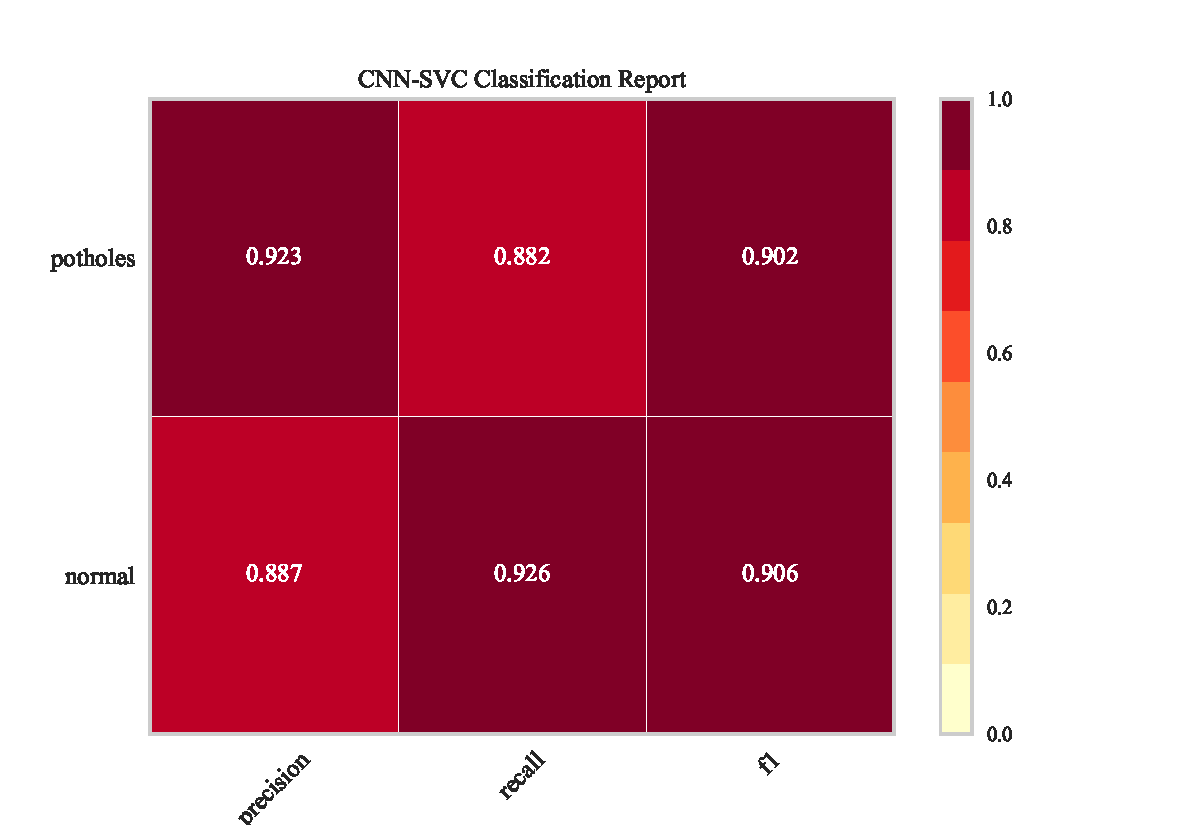
\includegraphics[width=0.96\linewidth]{[CNN-SVC]分类报告.pdf}
		\caption{CNN-SVM分类报告图}
		\label{fig:CNN-SVM分类报告图}
	\end{minipage}
	%\qquad
	\begin{minipage}{0.48\linewidth}
		\centering
		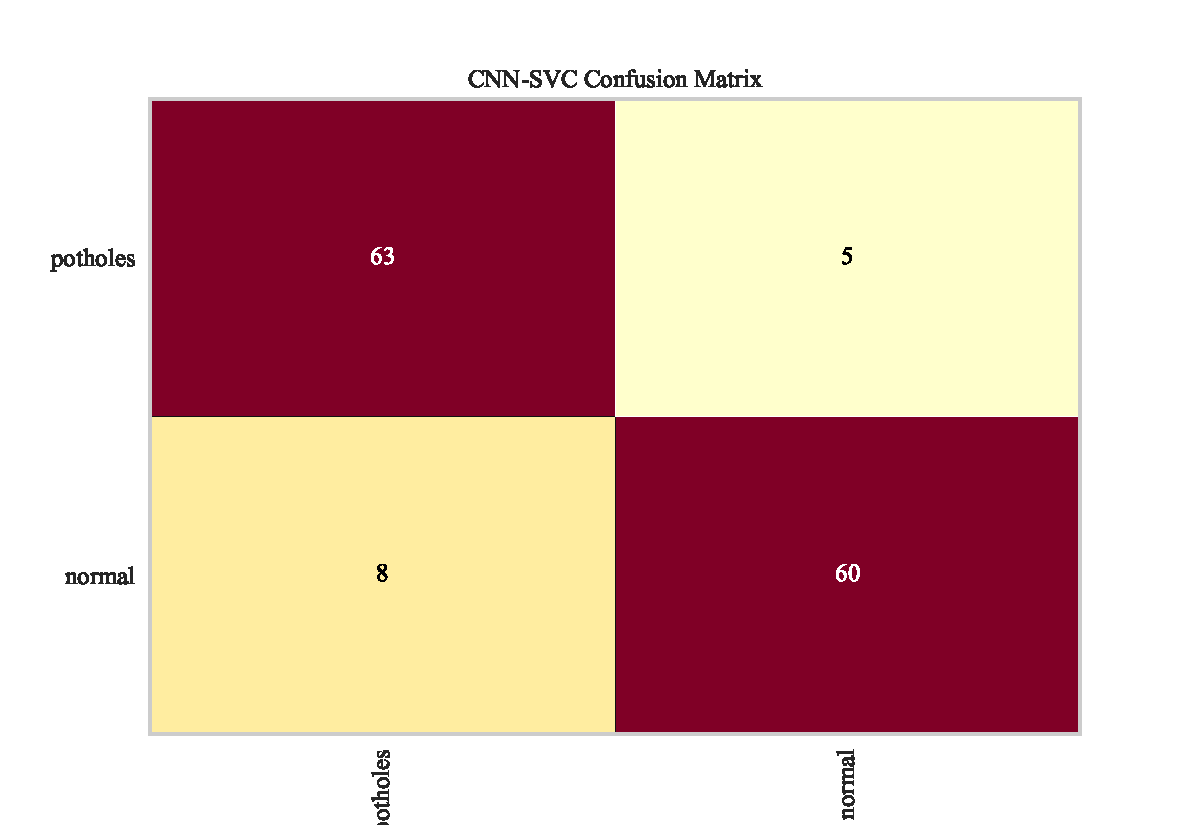
\includegraphics[width=0.96\linewidth]{[CNN-SVC]混淆矩阵热力图.pdf}
		\caption{CNN-SVM混淆矩阵热力图}
		\label{fig:CNN-SVM混淆矩阵热力图}
	\end{minipage}
\end{figure}

同时,我们还绘制模型的ROC/AUC曲线以及精确率-召回率曲线,分别如\textcolor{blue}{\cref{fig:CNN-SVM ROC/AUC曲线}}与\textcolor{blue}{\cref{fig:CNN-SVM精确率召回率曲线}}所示。由图可知,该模型的ROC/AUC曲线主要分布在左上方,曲线下面积较大,即AUC值较高,为$0.90$;同时,该模型的精确率与召回率都位于较高的数值,说明该模型在对道路是否坑洼的识别上准确度高,模型效果较好。

\begin{figure}[H]
	\centering
	\begin{minipage}{0.48\linewidth}
		\centering
		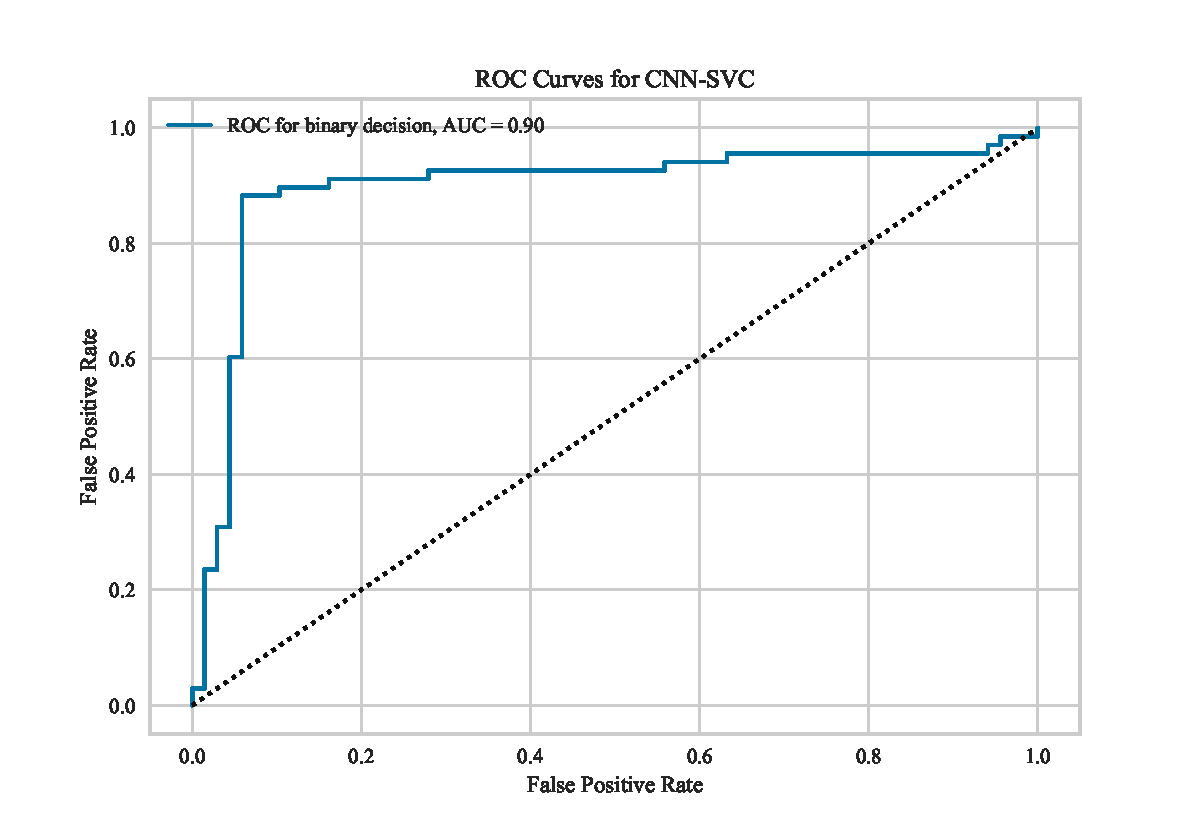
\includegraphics[width=0.96\linewidth]{[CNN-SVC]ROC曲线.pdf}
		\caption{CNN-SVM\,ROC曲线}
		\label{fig:CNN-SVM ROC/AUC曲线}
	\end{minipage}
	%\qquad
	\begin{minipage}{0.48\linewidth}
		\centering
		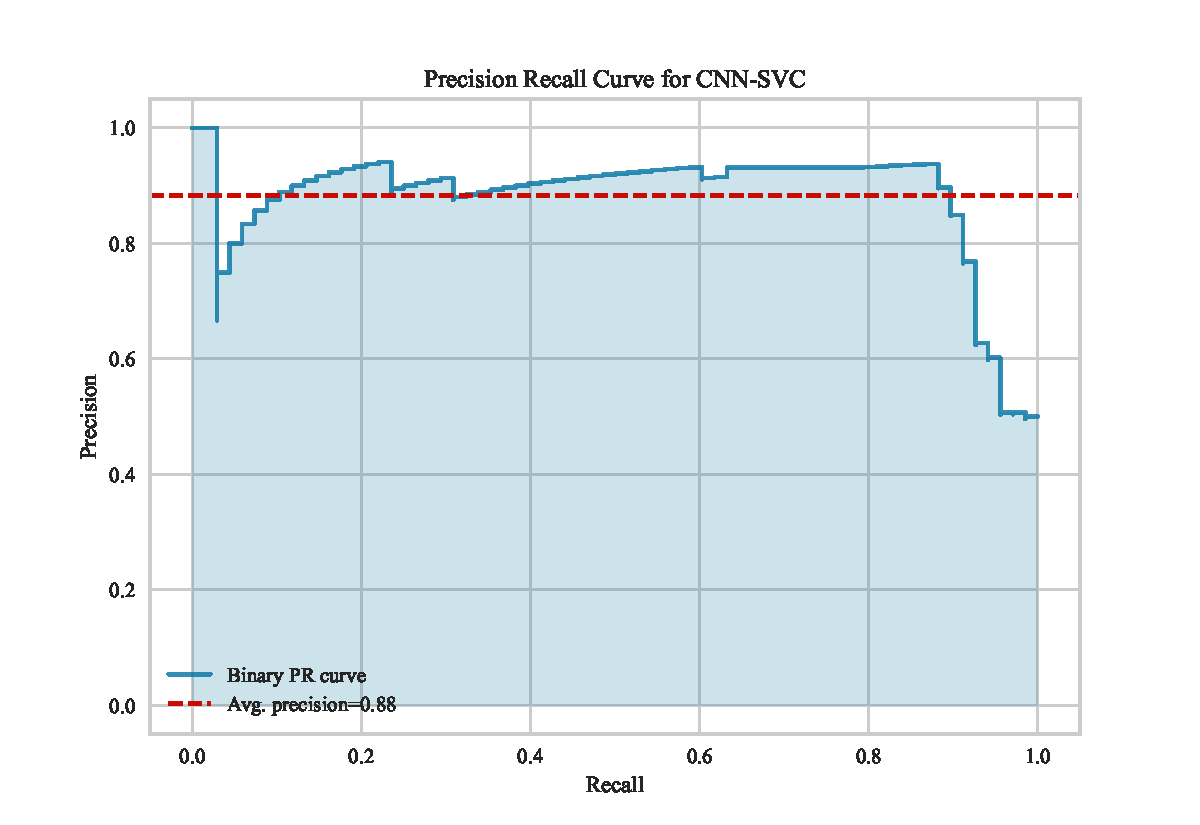
\includegraphics[width=0.96\linewidth]{[CNN-SVC]精确率召回率曲线.pdf}
		\caption{CNN-SVM精确率-召回率曲线}
		\label{fig:CNN-SVM精确率召回率曲线}
	\end{minipage}
\end{figure}
	\end{itemize}

	此外,我们还对该模型进行了五折交叉验证,具体结果为:
	\begin{equation}
		\boldsymbol{[0.96428571, 0.88888889, 0.88888889,0.85185185, 0.92592593]}\nonumber
	\end{equation}
	因而,可以得到该模型的准确率在置信度为$95\,\%$的水平下,置信区间为$\left[82\,\%, 98\,\%\right]$。
	\subsubsection{模型对比}
	未选择最优模型,我们依据\textcolor{blue}{\nameref{模型效果}}部分,将各模型指标整理至一张表格中,如\textcolor{blue}{\cref{tab:模型效果对比}}所示。同时结合\textcolor{blue}{\cref{fig:CNN-SVM分类报告图}}\textasciitilde\textcolor{blue}{\cref{fig:CNN-SVM精确率召回率曲线}},我们可以发现,在三者中,CNN-SVM模型的效果最优,其各项指标均较优秀。

\begin{table}[htbp]
	\centering
	\caption{模型效果对比}
	\scalebox{0.9}{
	  \begin{tabular}{ccccc}
	  \toprule
	  \textbf{指标} & \textbf{计算维度} & \textbf{PCA-SVM} & \textbf{CNN} & \textbf{CNN-SVM} \\
	  \midrule
	  \multirow{4}[2]{*}{\textbf{precision}} & 0:potholes & 0.50  & \textbf{0.90 } & 0.89  \\
			& 1:normal & 0.89  & 0.88  & \textbf{0.92 } \\
			& macro & 0.70  & 0.89  & \textbf{0.91 } \\
			& weighted & 0.84  & 0.89  & \textbf{0.91 } \\
	  \midrule
	  \multirow{4}[2]{*}{\textbf{recall}} & 0:potholes & 0.25  & 0.88  & \textbf{0.93 } \\
			& 1:normal & \textbf{0.96 } & 0.90  & 0.88  \\
			& macro & 0.61  & 0.89  & \textbf{0.90 } \\
			& weighted & 0.87  & 0.89  & \textbf{0.90 } \\
	  \midrule
	  \multirow{4}[2]{*}{\textbf{f1-score}} & 0:potholes & 0.33  & 0.89  & \textbf{0.91 } \\
			& 1:normal & \textbf{0.93 } & 0.89  & 0.90  \\
			& macro & 0.63  & 0.89  & \textbf{0.90 } \\
			& weighted & 0.85  & 0.89  & \textbf{0.90 } \\
	  \midrule
	  \textbf{accuracy} & 整体    & 0.87  & 0.89  & \textbf{0.90 } \\
	  \midrule
	  $\boldsymbol{T}$     & 共计    & 6\,m 8\,s 197\,ms & \textbf{5\,m 27\,s 323\,ms} & 6\,m 15\,s 37\,ms \\
	  \bottomrule
	  \end{tabular}}
	\label{tab:模型效果对比}
\end{table}

	\subsection{未知数据集的预测}
	对于该问题,具体处理代码见\textbf{附录-C.7,Predict [预测]}。我们按以下步骤进行处理:
	\begin{itemize}
		\item \textbf{读取已建立、训练完成的CNN-SVM模型}:将上述CNN-SVM模型利用keras及pickle库读取;
		\item \textbf{读取未知数据集}:将未知数据集的图像数据及其文件名(包括后缀名)一并读入,方便后续结果的输出,共计4942张图像;
		\item \textbf{对未知数据集进行预处理}:为了准确预测,需要将该数据集格式转换为前期训练模型输入的格式,避免预测错误。
		\item \textbf{对未知数据集进行预测}:首先传入CNN卷积神经网络,对数据集的特征进行提取;之后将提取的特征数据集传入SVM支持向量机中,进行预测;
		\item \textbf{结果查看}:经过上述步骤,将文件名与预测结果一一对应转为表格数据,方便查看;通过预测,模型在4942张图像中,识别出坑洼道路为3765张,识别为正常道路为1177张。
		\item \textbf{保存结果}:确认无误后,将上述表格输出为“test\_result.csv”文件。
	\end{itemize}
	\section{模型的评价与推广}
	\subsection{模型的评价}
	\begin{itemize}
		\item \textbf{模型的优点}
		\begin{enumerate}
			\item 未完全套用深度学习及传统机器学习模型,而是将CNN与SVM结合,使得模型能够处理非线性且稀疏数据并且对于权重的处理更加准确;
			\item 建立不同的模型进行对比分析,使结果更加准确;
			\item 在图像文件预处理时,对数据进行了人为再分类,使数据更准确有效;
			\item 在图像数据预处理时,对训练集进行高斯、双边滤波与旋转增强,提升模型的泛化能力;
			\item 由于所给原数据集分类样本不平衡,我们使用了采样的方法,适当增加数据集,使得原数据集为新数据集的子集,且分类样本平衡化。
		\end{enumerate}
		\item \textbf{模型的缺点}
		\begin{enumerate}
			\item 在对训练集进行数据增强时,仅使用了三种增强方法,在对特征进行学习时可能会有所遗漏;
			\item 由于所给原数据集分类样本不平衡,我们使用了采样的方法,适当增加数据集,使得原数据集为新数据集的子集,且分类样本平衡化。然后,该方法成本较高,对于数据集较少的任务,难以推广使用。
		\end{enumerate}
		\item \textbf{模型的改进}
		\begin{enumerate}
			\item 由于所给原数据集分类样本不平衡,除本文方法外,还可在模型中使用可选度量法和代价敏感学习进行解决\textcolor{blue}{\cite{数据挖掘导论}};
			\item 对于CNN神经网络,可选择其他更适合本题的架构使模型更加精确;
			\item 在进行预测时,可以结合优化算法,如贝叶斯调优进一步优化模型超参数,以提高预测精度。其主要方法为:利用已知的超参数$x$和模型结果$y$来拟合一个代理模型,再利用采集函数选择下一个最优$\left(x,y\right)$,并用此新的$\left(x,y\right)$来优化代理模型,重复上述过程,最终得到调优后的参数,其算法伪代码如\textcolor{blue}{Algorithm \ref{贝叶斯优化}}所示。
			\item 对于本文的SVM模型,我们可用其他分类效果更好的模型,如Stacking多模型融合集成学习。
		\end{enumerate}
	\end{itemize}

	\scalebox{0.85}{
	\begin{algorithm}[H]
		\label{贝叶斯优化}
		\KwIn{初始化点个数$n_0$,最大迭代次数$N$,代理模型$g\left(x\right)$,采集函数$\alpha\left(x|D\right)$}
		\KwOut{最优候选评估点:$\left\{x^{*},y^{*}\right\}$}
		\textbf{Step 1:}随机初始化$n_0$点$X_{\text{init}}=\left\{x_0,x_1,\cdots,x_{n_0-1}\right\}$\
		
		\textbf{Step 2:}获取其对应的函数值$f\left(X_\text{init}\right)$,初始点集$D_0=\left\{X_\text{init},f\left(X_\text{init}\right)\right\}$,令$t=n_0$,$D_{t-1}=D_0$\

		\While{t<N}{
			\textbf{Step 3:}根据当前获得的点集$D_{t-1}$,构建代理模型$g\left(x\right)$\
			
			\textbf{Step 4:}基于代理模型$g\left(x\right)$,最大化采集函数$\alpha\left(x|D_{t-1}\right)$,获得下一个评估点:$x_t=\text{argmin}\,\alpha\left(x|D_{t-1}\right)$\
			
			\textbf{Step 5:}获得评估点$x_t$的函数值$f\left(x_t\right)$,将其加入到当前评估点集合中:$D_t=D_{t-1}U\left\{x_t,f\left(x_t\right)\right\}$,转\textbf{Step 3}\
		}

		\KwResult{最优候选评估点:$\left\{x^{*},y^{*}\right\}$}
		\caption{贝叶斯优化框架}
	\end{algorithm}}
	\subsection{模型的推广}
	此模型具备处理具有复杂特征图像的能力,且能够较好地进行分类,因此除了判别道路坑洼与否外,我们也可将此其应用于重大基础设施建设前的勘探过程中,对工程建设地区的形进行判别,准确且快速地确定该地区是否适合建设该工程。以此类推,除了工程方面,此模型还可应用于交通预警,此模型适用于各地交管局及城市建设市政管理部门。在一定程度上改善了当前的预警机制,为减少民众财产损失做出了贡献。
	\newpage
	
	\phantomsection
	\addcontentsline{toc}{section}{\textbf{参考文献}}
	\begin{spacing}{1.08}
	\begin{thebibliography}{99}
	\bibitem{曹江华}曹江华. 复杂背景下非结构化道路可行驶区域检测研究[D].浙江科技学院,2021.

	\bibitem{刘建新}刘建新,史志仙.概率论与数理统计[M].北京:高等教育出版社,2016:115.

	\bibitem{汪海燕}汪海燕,黎建辉,杨风雷.支持向量机理论及算法研究综述[J].计算机应用研究,2014,31(05):1281-1286.

	\bibitem{张松兰}张松兰,王鹏,徐子伟.基于统计相关的缺失值数据处理研究[J].统计与决策,2016,No.456(12):13-16.

	\bibitem{李莎}李莎.基于改进卷积神经网络的上市企业财务风险预测研究[J].现代信息科技,2023,7(20):111-115.

	\bibitem{孟琪琳}孟琪琳,窦燕.基于EMD-CNN-LSTM模型的铁路客运量短期预测研究[J/OL].铁道运输与经济:1-9[2023-10-30].

	\bibitem{ZHANGP}ZHANG P,FANG Y.Research on text classification algorithm based on machine learning[J].Journal of Physics Conference Series,2020,1624:042010.

	\bibitem{李毅泉}李毅泉. 基于注意力机制的显著区域提取研究和实现[D].北京交通大学,2007.

	\bibitem{何铠}何铠,管有庆,龚锐.基于深度学习和支持向量机的文本分类模型[J].计算机技术与发展,2022,32(07):22-27.

	\bibitem{刘幸倩}刘幸倩. 基于注意力增强卷积神经网络的滚动轴承故障诊断方法研究[D].东北石油大学,2023.

	\bibitem{损失函数}CSDN.损失函数:categorical\_crossentropy[EB/OL].\url{https://blog.csdn.net/qq_40661327/article/details/107034575}.

	\bibitem{模型评测}知乎.模型评测:PRECISION、RECALL、F1-score[EB/OL].\url{https://zhuanlan.zhihu.com/p/519982682}.

	\bibitem{Tharwat}A.Tharwat, Applied Computing and Informatics (2018). \url{https://doi.org/10.1016/j.aci.2018.08.003}.

	\bibitem{Yellowbrick}Yellowbrick.Precision-Recall Curves - Yellowbrick v1.5 documentation[EB/OL].\url{https://www.scikit-yb.org/en/latest/api/classifier/prcurve.html}.

	\bibitem{数据挖掘导论}Tan P N, Steinbach M, Karpatne A, et al. Introduction to Data Mining[M]. Pearson, 2019:389.
	\end{thebibliography}
	\end{spacing}
	\newpage

	\phantomsection
	\addcontentsline{toc}{section}{\textbf{附\hspace{2pc}录}}

	% \appendix
	% \ctexset{section={format={\zihao{-4}\heiti\raggedright}}}
	\begin{center}
		\heiti\zihao{4} 附\hspace{2pc}录
	\end{center}

% \phantomsection
% \addcontentsline{toc}{subsection}{[A]图示}
% 	% \section*{[A]图表}
% 	\noindent{\heiti [A]图示}
% \newpage
% \phantomsection
% \addcontentsline{toc}{subsection}{[B]支撑文件列表}
% 	% \section*{[B]支撑文件列表}
	\noindent{\heiti [A]支撑文件列表}
	~\\

	支撑文件列表如下(列表中不包含原始数据集):
	% Table generated by Excel2LaTeX from sheet 'Sheet2'
	\begin{table}[H]
		\centering
		\scalebox{0.9}{
		  \begin{tabular}{cc}
		  \toprule
		  \textbf{文件夹名} & \textbf{描述} \\
		  \midrule
		  html文件 & 包括所有解决问题的源程序运行结果 \\
		  ipynb文件 & 包括所有解决问题的源程序源代码 \\
		  py文件  & 包括所有解决问题的源程序输出python文件 \\
		  models文件  & 已训练好的模型文件 \\
		  test\_result.csv  & 已训练模型识别测试集坑洼图像结果 \\
		  \bottomrule
		  \end{tabular}}
	\end{table}
  
\newpage
% \phantomsection
% \addcontentsline{toc}{subsection}{[C]使用的软件、环境}
	% \section*{[C]使用的软件、环境}
	\noindent{\heiti [B]使用的软件、环境}
	% ~\\

	\textbf{B.1 使用的软件及版本}
	\begin{itemize}
		\item TeX Live 2022
		\item Visual Studio Code 1.83.1
		\item WPS Office 2023秋季更新(15398)
		\item Python 3.10.4 [MSC v.1929 64 bit (AMD64)] on win32
		\item Pycharm 2023.2.3 (Professional Edition)
	\end{itemize}
	
	\textbf{B.2 模型训练所用计算机配置}
	\begin{itemize}
		\item Intel(R) Core(TM) i5-10200H CPU @ 2.40GHz
		\item NVIDIA GeForce GTX 1650 Ti
		\item NVIDIA CUDA 11.7.102 driver
		\item 16.0 GB RAM
		\item Windows 10 家庭中文版 22H2
	\end{itemize}

	\textbf{Python环境下所用使用到的库及其版本}
\begin{table}[htbp]
	\centering
	\setlength{\aboverulesep}{0pt}
	\setlength{\belowrulesep}{0pt}
	\scalebox{0.9}{
	  \begin{tabular}{cc||cc}
	  \toprule
	  \textbf{库}     & \textbf{版本}    & \textbf{库}     & \textbf{版本} \\
	  \midrule
	  collections & 内置库   & jupyterlab-widgets & 3.0.9 \\
	  opencv-python & 4.8.1.78 & keras & 2.14.0 \\
	  h5py  & 3.10.0 & matplotlib & 3.8.0 \\
	  jupyter & 1.0.0 & numpy & 1.26.1 \\
	  jupyter\_client & 8.5.0 & os    & 内置库 \\
	  jupyter-console & 6.6.3 & pandas & 2.1.2 \\
	  jupyter\_core & 5.4.0 & pickle & 内置库 \\
	  jupyter-events & 0.8.0 & random & 内置库 \\
	  jupyter-lsp & 2.2.0 & shutil & 内置库 \\
	  jupyter\_server & 2.9.1 & sklearn & 1.3.2 \\
	  jupyter\_server\_terminals & 0.4.4 & tensorflow & 2.14.0 \\
	  jupyterlab & 4.0.7 & warnings & 内置库 \\
	  jupyterlab-pygments & 0.2.2 & yellowbrick & 1.50  \\
	  jupyterlab\_server & 2.25.0 &       &  \\
	  \bottomrule
	  \end{tabular}}
\end{table}

\newpage
% \phantomsection
% \addcontentsline{toc}{subsection}{[D]问题解决源程序}
	% \section*{[D]问题解决源程序}
\noindent{\heiti [C]问题解决源程序}

\textbf{C.1 Data Preprocessing [数据预处理]}
\begin{python}
#!/usr/bin/env python
# coding: utf-8

# In[1]:


import os
import shutil

# 指定目录"DATA"
path = "DATA"

# 在"DATA"文件夹中创建"normal"和"potholes"文件夹
os.mkdir(os.path.join(path, "normal"))
os.mkdir(os.path.join(path, "potholes"))

# 读取"DATA"文件夹,若文件名中含有"normal",则将其放置于"normal"文件夹中,否则放置于"potholes"文件夹中
files = os.listdir(path)
for file in files:
    if "normal" in file:
        shutil.move(os.path.join(path, file), os.path.join(path, "normal"))
    else:
        shutil.move(os.path.join(path, file), os.path.join(path, "potholes"))

\end{python}

\textbf{C.2 Comparative Analysis of Normal and Potholes [正常与坑洼道路的比较分析]}
\begin{python}
#!/usr/bin/env python
# coding: utf-8

# In[1]:


import cv2
import numpy as np
import matplotlib.pyplot as plt

# In[2]:


normalImg = cv2.imread('DATA\\normal\\normal133.jpg')
potholesImg = cv2.imread('DATA\\potholes\\potholes1.jpg')

# In[3]:


plt.rcParams['font.sans-serif'] = ['Times New Roman']
plt.rcParams['axes.unicode_minus'] = False


# In[4]:


def cv_show(img):
    b, g, r = cv2.split(img)
    img = cv2.merge([r, g, b])
    plt.imshow(img)


# In[5]:


cv_show(normalImg)

# In[6]:


cv_show(potholesImg)

# In[7]:


color = ('b', 'g', 'r')

for i, col in enumerate(color):
    histr = cv2.calcHist([normalImg], [i], None, [256], [0, 256])
    plt.plot(histr, color=col)

plt.legend(['Blue', 'Green', 'Red'])
plt.xlim([0, 256])
plt.xticks(fontsize=10)
plt.yticks(fontsize=10)
plt.title('(a) normal133.jpg', y=-0.2, fontsize=12)
plt.xlabel('Pixel Value', fontsize=11)
plt.ylabel('Number of Pixels', fontsize=11)
plt.savefig('Figures\\normal133RGB直方图.pdf', bbox_inches='tight')

# In[8]:


color = ('b', 'g', 'r')

for i, col in enumerate(color):
    histr = cv2.calcHist([potholesImg], [i], None, [256], [0, 256])
    plt.plot(histr, color=col)

plt.legend(['Blue', 'Green', 'Red'])
plt.xlim([0, 256])
plt.xticks(fontsize=10)
plt.yticks(fontsize=10)
plt.title('(b) potholes1.jpg', y=-0.2, fontsize=12)
plt.xlabel('Pixel Value', fontsize=11)
plt.ylabel('Number of Pixels', fontsize=11)
plt.savefig('Figures\\potholes1RGB直方图.pdf', bbox_inches='tight')

# In[9]:


plt.style.use('ggplot')
plt.hist(normalImg.ravel(), 256, [0, 256], color='grey')
plt.title('(a) normal133.jpg', y=-0.2, fontsize=12)
plt.xlabel('Pixel Value', fontsize=11)
plt.ylabel('Number of Pixels', fontsize=11)
plt.savefig('Figures\\normal133灰度直方图.pdf', bbox_inches='tight')

# In[10]:


plt.style.use('ggplot')
plt.hist(potholesImg.ravel(), 256, [0, 256], color='grey')
plt.title('(b) potholes1.jpg', y=-0.2, fontsize=12)
plt.xlabel('Pixel Value', fontsize=11)
plt.ylabel('Number of Pixels', fontsize=11)
plt.savefig('Figures\\potholes1灰度直方图.pdf', bbox_inches='tight')

# In[11]:


# 边缘检测
gray = cv2.cvtColor(normalImg, cv2.COLOR_BGR2GRAY)
edges = cv2.Canny(gray, 100, 200)
plt.imshow(edges, cmap='gray')
plt.title('(a) normal133.jpg', y=-0.2, fontsize=12)
plt.savefig('Figures\\normal133边缘检测.pdf', bbox_inches='tight')

# In[12]:


# 边缘检测
gray = cv2.cvtColor(potholesImg, cv2.COLOR_BGR2GRAY)
edges = cv2.Canny(gray, 100, 200)
plt.imshow(edges, cmap='gray')
plt.title('(b) potholes1.jpg', y=-0.2, fontsize=12)
plt.savefig('Figures\\potholes1边缘检测.pdf', bbox_inches='tight')

# In[13]:


plt.imshow(normalImg)
plt.colorbar()
plt.title('(a) normal133.jpg', y=-0.3, fontsize=12)
plt.savefig('Figures\\normal133热力图.pdf')

# In[14]:


plt.imshow(potholesImg)
plt.colorbar()
plt.title('(b) potholes1.jpg', y=-0.3, fontsize=12)
plt.savefig('Figures\\potholes1热力图.pdf')

# In[15]:


# 阈值分割
hsv = cv2.cvtColor(normalImg, cv2.COLOR_BGR2HSV)
lower_blue = np.array([90, 50, 50])
upper_blue = np.array([130, 255, 255])
mask = cv2.inRange(hsv, lower_blue, upper_blue)
plt.imshow(mask, cmap='gray')
plt.title('(a) normal133.jpg', y=-0.2, fontsize=12)
plt.savefig('Figures\\normal133阈值分割.pdf', bbox_inches='tight')

# In[16]:


# 阈值分割
hsv = cv2.cvtColor(potholesImg, cv2.COLOR_BGR2HSV)
lower_blue = np.array([90, 50, 50])
upper_blue = np.array([130, 255, 255])
mask = cv2.inRange(hsv, lower_blue, upper_blue)
plt.imshow(mask, cmap='gray')
plt.title('(b) potholes1.jpg', y=-0.2, fontsize=12)
plt.savefig('Figures\\potholes1阈值分割.pdf', bbox_inches='tight')

# In[17]:


# 转换为灰度图像
gray = cv2.cvtColor(normalImg, cv2.COLOR_BGR2GRAY)
# 二值化
ret, binary = cv2.threshold(gray, 0, 255, cv2.THRESH_BINARY | cv2.THRESH_OTSU)
# 轮廓检测
contours, hierarchy = cv2.findContours(binary, cv2.RETR_TREE, cv2.CHAIN_APPROX_SIMPLE)
# 绘制轮廓
cv2.drawContours(normalImg, contours, -1, (0, 0, 255), 3)

plt.subplot(1, 2, 1)
plt.title('(a) Original', y=-0.4, fontsize=12)
plt.imshow(normalImg)
plt.subplot(1, 2, 2)
plt.imshow(binary, cmap='gray')
plt.title('(b) Contours', y=-0.4, fontsize=12)
plt.savefig('Figures\\normal133轮廓检测.pdf', bbox_inches='tight')

# In[18]:


# 转换为灰度图像
gray = cv2.cvtColor(potholesImg, cv2.COLOR_BGR2GRAY)
# 二值化
ret, binary = cv2.threshold(gray, 0, 255, cv2.THRESH_BINARY | cv2.THRESH_OTSU)
# 轮廓检测
contours, hierarchy = cv2.findContours(binary, cv2.RETR_TREE, cv2.CHAIN_APPROX_SIMPLE)
# 绘制轮廓
cv2.drawContours(potholesImg, contours, -1, (0, 0, 255), 3)

plt.subplot(1, 2, 1)
plt.title('(a) Original', y=-0.4, fontsize=12)
plt.imshow(potholesImg)
plt.subplot(1, 2, 2)
plt.imshow(binary, cmap='gray')
plt.title('(b) Contours', y=-0.4, fontsize=12)
plt.savefig('Figures\\potholes1轮廓检测.pdf', bbox_inches='tight')

\end{python}

\textbf{C.3 Random Plot Images [随机展现正常与坑洼道路图像]}
\begin{python}
#!/usr/bin/env python
# coding: utf-8

# In[1]:


import pathlib
import matplotlib.pyplot as plt
from keras.preprocessing.image import ImageDataGenerator


# In[2]:


dataDirectory = pathlib.Path('DATA\\')
classNames = [item.name for item in dataDirectory.glob('*')][:2]
classNames


# In[3]:


dataAdd = 'DATA' 
normalAdd = 'DATA\\normal'
potholesAdd = 'DATA\\potholes'

# 定义一个数据生成器,用于处理图像数据,并对数据进行归一化处理。同时,将数据集的20%作为验证数据,而其余80%用于训练
dataImageDataGenerator = ImageDataGenerator(rescale = 1/255., validation_split = 0.2)
dataTrain = dataImageDataGenerator.flow_from_directory(dataAdd, target_size = (224, 224), batch_size = 32, subset = 'training', class_mode = 'binary')
dataVal = dataImageDataGenerator.flow_from_directory(dataAdd, target_size = (224, 224), batch_size = 32, subset = 'validation', class_mode = 'binary')


# In[4]:


def random_plot_images():
    images, labels = dataTrain.next()
    labels = labels.astype('int32')
    i = 1

    plt.figure(figsize = (10, 10))
    
    for image, label in zip(images, labels):
        plt.subplot(4, 5, i)
        plt.imshow(image)
        if label == 0:
            plt.title(classNames[label],fontname='Times New Roman', fontsize=12, color='blue')
        else:
            plt.title(classNames[label],fontname='Times New Roman', fontsize=12, color='red')
        plt.axis('off')
        i += 1
        if i == 21:
            break

    plt.tight_layout()       
    plt.savefig('Figures\\图像数据观测.pdf')


random_plot_images()

\end{python}

\textbf{C.4 PCA-SVM [PCA降维、网格调优的支持向量机]}
\begin{python}
#!/usr/bin/env python
# coding: utf-8

# In[1]:


import os
import cv2
import numpy as np
import collections
from sklearn import svm
import matplotlib.pyplot as plt
from sklearn.decomposition import PCA
from sklearn.metrics import accuracy_score
from keras.preprocessing.image import ImageDataGenerator


# In[2]:


# 加载图像数据
def load_img():
    inputImg, inputLabel = [], []
    resize = (224, 224)
    for dirname, _, filenames in os.walk('DATA\\'):
        for filename in filenames:
            photo_path = os.path.join(dirname, filename)
            photo_class = dirname.split('\\')[-1]
            try:
                read_im = cv2.imread(photo_path)
                inputImg.append(cv2.resize(read_im, resize))
                # potholes == 0
                if photo_class == 'potholes':
                    inputLabel.append(0)
                # normal == 1
                elif photo_class == 'normal':
                    inputLabel.append(1)
            except:
                print(photo_path)
    return inputImg, inputLabel


inputImg, inputLabel = load_img()

# In[3]:


# 计算inputLabel中各类别的数量
counter = collections.Counter(inputLabel)
counter


# In[4]:


# 随机划分训练集和测试集,比例为test_prop,x为图像数据,y为标签
def train_test_split(test_prop, inputImg, inputLabel):
    test_size = int(np.floor(test_prop * len(inputLabel)))
    # 随机数
    np.random.seed(202310)
    test_index = np.random.choice(len(inputLabel), size=test_size, replace=False)
    # 划分
    train_x, test_x, train_y, test_y = np.delete(inputImg, test_index, axis=0), np.take(inputImg, test_index, axis=0), np.delete(inputLabel, test_index, axis=0), np.take(inputLabel, test_index, axis=0)
    # 返回图像和标签的训练集和测试集
    return train_x, test_x, train_y, test_y, test_index


train_x, test_x, train_y, test_y, test_index = train_test_split(0.2, inputImg, inputLabel)


# In[5]:


# opencv滤波增加训练集
def opencv_blur(inputImg, inputLabel):
    inputLabelNew = inputLabel.copy()
    inputImgNew = inputImg.copy()
    for i in range(len(inputImg)):
        im = inputImg[i]
        im = im.astype('uint8')
        imLbl = [inputLabel[i]]

        # 高斯滤波
        imgGaussian = cv2.GaussianBlur(im, (5, 5), 0)
        # 双边滤波
        imgBilateral = cv2.bilateralFilter(im, 9, 75, 75)

        # 添加到训练集中
        inputImgNew = np.append(inputImgNew, [imgGaussian, imgBilateral], axis=0)
        inputLabelNew = np.append(inputLabelNew, imLbl * 2, axis=0)
    return inputImgNew, inputLabelNew


inputImgNew, inputLabelNew = opencv_blur(train_x, train_y)


# In[6]:


# 图像增强,在原有的训练集上进行图像增强
def append_img(inputImg, inputLabel, imgIterator):
    inputLabelNew = inputLabel.copy()
    inputImgNew = inputImg.copy()
    for i in range(len(imgIterator)):
        im = imgIterator[i]
        im = im.astype('uint8')
        imLbl = [inputLabel[i]]
        inputImgNew = np.append(inputImgNew, im, axis=0)
        inputLabelNew = np.append(inputLabelNew, imLbl, axis=0)
    return inputImgNew, inputLabelNew


# In[7]:


# 旋转 + 30 deg
rotate_data_generartor = ImageDataGenerator(rotation_range=30)
imgIterator = rotate_data_generartor.flow(train_x, batch_size=1, shuffle=False)
inputImgNew, inputLabelNew = append_img(inputImgNew, inputLabelNew, imgIterator)

# In[8]:


# 计算inputLabelNew中各类别的数量
counter = collections.Counter(inputLabelNew)
counter


# In[9]:


def plot_img(inputImgNew, inputLabelNew):
    plt.figure(figsize=(12, 5))
    i = 1
    for image, label in zip(inputImgNew, inputLabelNew):
        if i <= 5:
            if label == 1:
                plt.subplot(2, 5, i)
                plt.imshow(image)
                plt.title('normal', fontname='Times New Roman', fontsize=12, color='blue')
                plt.axis('off')
                i += 1
        elif 5 < i < 11:
            if label == 0:
                plt.subplot(2, 5, i)
                plt.imshow(image)
                plt.title('potholes', fontname='Times New Roman', fontsize=12, color='red')
                plt.axis('off')
                i += 1
        else:
            break
    plt.savefig('Figures\\PCA-SVM训练样本.pdf', bbox_inches='tight')


plot_img(inputImgNew, inputLabelNew)

# In[10]:


nx, ny, nz = train_x.shape[1], train_x.shape[2], train_x.shape[3]
train_x_nn, test_x_nn = inputImgNew, test_x
train_x = inputImgNew.reshape((inputImgNew.shape[0], nx * ny * nz)) / 255
test_x = test_x.reshape((test_x.shape[0], nx * ny * nz)) / 255
train_y = inputLabelNew.reshape((inputLabelNew.shape[0], 1))
test_y = test_y.reshape((test_y.shape[0], 1))

# In[11]:


im_pca = PCA()
im_pca.fit(train_x)
variance_explained_list = im_pca.explained_variance_ratio_.cumsum()

# In[12]:


test_x_pca = im_pca.transform(test_x)
train_x_pca = im_pca.transform(train_x)


# In[13]:


# SVM网格调优
def svm_grid_search(C, kernel, train_x, train_y):
    accuracy_score_list = []

    for c in C:
        svmClassifier = svm.SVC(C=c, kernel=kernel)
        svmClassifier.fit(train_x, train_y.ravel())
        pred_y = svmClassifier.predict(train_x)
        accuracy = accuracy_score(train_y, pred_y)
        accuracy_score_list.append(accuracy)
        print('Regularization parameters: {:.2f},Accuracy:{:.4f}'.format(c, accuracy))

    max_accurarcy_id = accuracy_score_list.index(max(accuracy_score_list))
    return C[max_accurarcy_id]


C, kernel = [0.1 * i for i in range(1, 30)], 'rbf'
opt_C = svm_grid_search(C, kernel, train_x_pca, train_y)

# In[14]:


svmClassifier = svm.SVC(C=opt_C, kernel='rbf')
svmClassifier.fit(train_x_pca, train_y.ravel())
pred_y = svmClassifier.predict(test_x_pca)
accuracy = accuracy_score(test_y, pred_y)
print('Test Accuracy: {:2.2f}%'.format(accuracy * 100))

# In[15]:


# 分类报告
from sklearn.metrics import classification_report

print(classification_report(test_y, pred_y))

# In[16]:


# 保存模型
import pickle

with open('Models\\PCA.pkl', 'wb') as f:
    pickle.dump(im_pca, f)
with open('Models\\PCA-SVM.pkl', 'wb') as f:
    pickle.dump(svmClassifier, f)
f.close()

\end{python}

\textbf{C.5 CNN [卷积神经网络]}
\begin{python}
#!/usr/bin/env python
# coding: utf-8

# In[1]:


import os
import cv2
import h5py
import warnings
import numpy as np
import collections
import random as rn
import matplotlib.pyplot as plt
from keras.models import Sequential
from keras.utils import to_categorical
from keras.layers import Conv2D, MaxPooling2D
from sklearn.preprocessing import LabelEncoder
from keras.layers import Dense, Flatten, Dropout
from sklearn.model_selection import train_test_split

warnings.filterwarnings('always')
warnings.filterwarnings('ignore')

# In[2]:


imagePath = []
for dirname, _, filenames in os.walk('DATAX\\'):
    # 统计DATAX文件夹下子文件夹下的图片数量
    print(dirname, len(filenames))
    for filename in filenames:
        path = os.path.join(dirname, filename)
        imagePath.append(path)

len(imagePath)

# In[3]:


IMG_SIZE = 128
X = []
y = []
for image in imagePath:
    try:
        img = cv2.imread(image, cv2.IMREAD_COLOR)
        img = cv2.resize(img, (IMG_SIZE, IMG_SIZE))
        X.append(np.array(img))
        if image.startswith('DATAX\\normal'):
            y.append('normal')
        else:
            y.append('potholes')
    except:
        pass

# In[4]:


fig, ax = plt.subplots(2, 5)
plt.subplots_adjust(bottom=0.3, top=0.7, hspace=0)
fig.set_size_inches(15, 12.5)

plt.rcParams['font.sans-serif'] = ['Times New Roman']
plt.rcParams['axes.unicode_minus'] = False

for i in range(2):
    for j in range(5):
        l = rn.randint(0, len(y))
        ax[i, j].imshow(X[l][:, :, ::-1])
        if y[l] == 'normal':
            ax[i, j].set_title(y[l], color='blue')
        else:
            ax[i, j].set_title(y[l], color='red')
        ax[i, j].set_aspect('equal')

plt.savefig('Figures\\CNN训练样本.pdf', bbox_inches='tight')

# In[5]:


# 统计y中各类别的数量
collections.Counter(y)

# In[6]:


le = LabelEncoder()
Y = le.fit_transform(y)
Y = to_categorical(Y, 2)
X = np.array(X)

# In[7]:


y

# In[8]:


# Y中第一列:1表示normal,0表示potholes
Y

# In[9]:


# 划分训练集和测试集,测试集占比20%
x_train, x_test, y_train, y_test = train_test_split(X, Y, test_size=0.20, random_state=5)

# In[10]:


model = Sequential()
model.add(Conv2D(32, (5, 5), activation='relu', input_shape=(128, 128, 3)))
model.add(MaxPooling2D((2, 2)))
model.add(Conv2D(64, (3, 3), activation='relu'))
model.add(MaxPooling2D((2, 2)))
model.add(Conv2D(128, (3, 3), activation='relu'))
model.add(MaxPooling2D((2, 2)))
model.add(Conv2D(128, (3, 3), activation='relu'))
model.add(MaxPooling2D((2, 2)))
model.add(Conv2D(128, (3, 3), activation='relu'))
model.add(MaxPooling2D((2, 2)))

model.add(Flatten())
model.add(Dropout(0.4))
model.add(Dense(128, activation='relu'))
model.add(Dense(2, activation='softmax'))

# In[11]:


model.compile(optimizer='adam', loss='categorical_crossentropy', metrics=['accuracy'])
model.summary()

# In[12]:


history = model.fit(x_train, y_train, epochs=50, batch_size=12, verbose=2, validation_data=(x_test, y_test))

# In[13]:


loss, accuracy = model.evaluate(x_test, y_test)
print('Test Accuracy: {:2.2f}%'.format(accuracy * 100))

# In[14]:


plt.figure(figsize=(12, 5))
plt.subplot(1, 2, 1)
plt.title('(a) Accuracy and Loss', y=-0.2)
plt.plot(history.history['accuracy'])
plt.plot(history.history['loss'])
plt.xlabel('Epochs')
plt.ylabel('Accuracy')
plt.legend(['Accuracy', 'Loss'], loc='upper right')
plt.subplot(1, 2, 2)
plt.title('(b) Validation Accuracy and Loss', y=-0.2)
plt.plot(history.history['val_accuracy'])
plt.plot(history.history['val_loss'])
plt.xlabel('Epochs')
plt.ylabel('Validation Accuracy and Loss')
plt.legend(['Val Accuracy', 'Val Loss'], loc='upper left')
plt.savefig('Figures\\CNN训练结果.pdf', bbox_inches='tight')

# In[15]:


prediction = model.predict(x_test)
y_pred = np.argmax(prediction, axis=1)

# In[16]:


y_testA = y_test.astype(int)
y_testB = []
for i in y_testA:
    a = 1
    if i[0] == 1 and i[1] == 0:
        a = 0
    y_testB.append(a)

# In[17]:


# 分类报告
from sklearn.metrics import classification_report

print(classification_report(y_testB, y_pred))

# In[18]:


# 保存数据集为h5文件,包括X_train, X_test, y_train, y_test
h5f = h5py.File('Models\\CNNData.h5', 'w')
h5f.create_dataset('X_train', data=x_train)
h5f.create_dataset('X_test', data=x_test)
h5f.create_dataset('y_train', data=y_train)
h5f.create_dataset('y_test', data=y_test)
h5f.close()

# In[19]:


# 保存模型
model.save('Models\\CNN.h5')

\end{python}

\textbf{C.6 CNN-SVM [卷积神经网络与支持向量机]}
\begin{python}
#!/usr/bin/env python
# coding: utf-8

# In[1]:


import h5py
from sklearn.svm import SVC
import matplotlib.pyplot as plt
from keras.models import load_model
from yellowbrick.classifier import ROCAUC
from sklearn.metrics import accuracy_score
from sklearn.metrics import classification_report
from yellowbrick.classifier import ConfusionMatrix
from sklearn.model_selection import cross_val_score
from yellowbrick.classifier import ClassificationReport
from yellowbrick.classifier import PrecisionRecallCurve

# In[2]:


plt.rcParams['font.sans-serif'] = ['Times New Roman']

# In[3]:


# 加载CNN模型
CNNModel = load_model('Models\\CNN.h5')

# 加载CNN数据
with h5py.File('Models\\CNNData.h5', 'r') as file:
    X_train = file['X_train'][:]
    y_train = file['y_train'][:]
    X_test = file['X_test'][:]
    y_test = file['y_test'][:]

# 使用CNN提取特征
X_train_features = CNNModel.predict(X_train)
X_test_features = CNNModel.predict(X_test)

# In[4]:


# 使用SVM分类器
svm = SVC(kernel='rbf', random_state=0, gamma=2, C=1)
svm.fit(X_train_features, y_train[:, 0])

# In[5]:


y_pred = svm.predict(X_test_features)
print('Accuracy: %.2f%%' % (accuracy_score(y_test[:, 0], y_pred) * 100))
print(classification_report(y_test[:, 0], y_pred))

# In[6]:


# 分类报告可视化
visualizer = ClassificationReport(svm, classes=['potholes', 'normal'])
visualizer.fit(X_train_features, y_train[:, 0])
visualizer.score(X_test_features, y_test[:, 0])
plt.title('CNN-SVC Classification Report')
plt.savefig('Figures\\[CNN-SVC]分类报告.pdf')

# In[7]:


# yellowbrick绘制学混淆矩阵热力图
cm = ConfusionMatrix(svm, classes=['potholes', 'normal'])
cm.fit(X_train_features, y_train[:, 0])
cm.score(X_test_features, y_test[:, 0])
plt.title('CNN-SVC Confusion Matrix')
plt.savefig('Figures\\[CNN-SVC]混淆矩阵热力图.pdf')

# In[8]:


# yellowbrick绘制ROC曲线
visualizer = ROCAUC(svm, classes=['potholes', 'normal'], binary=True)
visualizer.fit(X_train_features, y_train[:, 0])
visualizer.score(X_test_features, y_test[:, 0])
plt.legend()
plt.xlabel('False Positive Rate')
plt.ylabel('False Positive Rate')
plt.title('ROC Curves for CNN-SVC')
plt.savefig('Figures\\[CNN-SVC]ROC曲线.pdf')

# In[9]:


# yellowbrick绘制精度-召回率曲线
visualizer = PrecisionRecallCurve(svm, classes=['potholes', 'normal'])
visualizer.fit(X_train_features, y_train[:, 0])
visualizer.score(X_test_features, y_test[:, 0])
plt.legend()
plt.xlabel('Recall')
plt.ylabel('Precision')
plt.title('Precision Recall Curve for CNN-SVC')
plt.savefig('Figures\\[CNN-SVC]精确率召回率曲线.pdf')

# In[10]:


# 使用五折交叉验证
scores = cross_val_score(svm, X_test_features, y_test[:, 0], cv=5)
# 输出交叉验证分数
print(scores)
print("Accuracy: %0.2f (+/- %0.2f)" % (scores.mean(), scores.std() * 2))

# In[11]:


import pickle

with open('Models\\CNN-SVM.pkl', 'wb') as f:
    pickle.dump(svm, f)
f.close()

\end{python}

\textbf{C.7 Predict [预测]}
\begin{python}
#!/usr/bin/env python
# coding: utf-8

# In[1]:


import os
import cv2
import pickle
import numpy as np
import pandas as pd
from keras.models import load_model

# In[2]:


CNNModel = load_model('Models\\CNN.h5')
with open('Models\\CNN-SVM.pkl', 'rb') as f:
    model = pickle.load(f)

# In[3]:


imagePath = []
for dirname, _, filenames in os.walk('DATAPre\\'):
    print(dirname, len(filenames))
    for filename in filenames:
        path = os.path.join(dirname, filename)
        imagePath.append(path)

len(imagePath)

# In[4]:


IMG_SIZE = 128
X = []
y = []
imgName = []
for image in imagePath:
    try:
        img = cv2.imread(image, cv2.IMREAD_COLOR)
        img = cv2.resize(img, (IMG_SIZE, IMG_SIZE))
        X.append(np.array(img))
        imgName.append(image.split('\\')[1])
    except:
        pass

# In[5]:


X = np.array(X)
X_train_features = CNNModel.predict(X)

# In[6]:


y_pred = model.predict(X_train_features)
df = pd.DataFrame({'fnames': imgName, 'label': y_pred})
df['label'] = df['label'].astype(int)
df

# In[7]:


df.to_csv('test_result.csv', index=False)

\end{python}

\textbf{C.8 Images Display [图像展示]}
\begin{python}
#!/usr/bin/env python
# coding: utf-8

# In[1]:


import cv2

img = cv2.imread("DATA\\potholes\\potholes1.jpg", cv2.IMREAD_COLOR)
img = cv2.resize(img, [256, 256])

Gaussian = cv2.GaussianBlur(img, (3, 3), 1)
Bilateral = cv2.bilateralFilter(img, 9, 75, 75)
Rotate = cv2.warpAffine(img, cv2.getRotationMatrix2D((img.shape[1] / 2, img.shape[0] / 2), 30, 1),
                        (img.shape[1], img.shape[0]))

cv2.imwrite("potholes1_Gaussian.jpg", Gaussian)
cv2.imwrite("potholes1_Bilateral.jpg", Bilateral)
cv2.imwrite("potholes1_Rotate.jpg", Rotate)

\end{python}
\end{document}